%-----------------------------------------------------------
%
%	Guide d'introduction à Java et WPILib
%	Par Étienne Beaulac
%	Ultime 5528
%
%-----------------------------------------------------------


\documentclass[12pt]{report}

%Code display, avant Babel !
%\usepackage{listings, minted}

\usepackage[francais]{babel}
\usepackage[utf8]{inputenc}
\usepackage[scaled]{helvet}
\renewcommand\familydefault{\sfdefault} 
%\usepackage{libertine}
%\usepackage{libertinust1math}
\usepackage[T1]{fontenc}
%\usepackage{lmodern}
%\usepackage{avant}

% Marges
\usepackage[margin=2cm]{geometry}

%Custom font sizes
\usepackage{anyfontsize}

%Tableau en français (et non table)
\usepackage{caption}
%\captionsetup[table]{name=Tableau}

%packages graphiques, mathématiques
\usepackage{amsfonts, amsmath, amssymb}

%Afficher des images avec includegraphics
\usepackage{graphicx}
\usepackage{adjustbox}

% Afficher des SVG
% Convertir un SVG en pdf_tex : inkscape -D -z --file=<NOM DU FICHIER.svg> --export-pdf=<OUTPUT.pdf> --export-latex
\usepackage{svg}

% Tableaux extensibles
\usepackage{tabularx}
\usepackage{booktabs}

%Image avec caption
\newcommand{\image}[2]{%

}

%Virgule pour nombres français
%\usepackage{icomma}

%Liens hypertextes
\usepackage{hyperref}
\hypersetup{
    colorlinks=true,
    linkcolor=blue,
    filecolor=magenta,      
    urlcolor=blue,
}

%Couleurs
\usepackage{xcolor}
\definecolor{ultRed}{RGB}{190,30,45}
\definecolor{ec-red}{RGB}{237,28,36}
\definecolor{ec-orange}{RGB}{255,127,39}
\definecolor{ec-yellow}{RGB}{255,242,0}
\definecolor{ec-green}{RGB}{34,177,76}
\definecolor{ec-purple}{RGB}{163,73,164}

%\usepackage{eso-pic}

%Nice code snippets
\usepackage[chapter]{minted}
\setminted[java]{%
	%linenos,
	autogobble
}

%Nice frames for minted
\usepackage{tcolorbox}
\tcbuselibrary{minted, skins, xparse, breakable}

\usepackage{tikz}
\usetikzlibrary{arrows.meta, shapes.geometric, positioning, decorations.pathreplacing}

% Ne pas copier les numéros de lignes de code
\usepackage{accsupp}
\newcommand\emptyaccsupp[1]{\BeginAccSupp{ActualText={}}#1\EndAccSupp{}}
%default definition is: \def\theFancyVerbLine{\rmfamily\tiny\arabic{FancyVerbLine}}
\let\theHFancyVerbLine\theFancyVerbLine% don't apply our patch to hyperref's version
%\def\theFancyVerbLine{\rmfamily\tiny\emptyaccsupp{\arabic{FancyVerbLine}}}
\def\theFancyVerbLine{\BeginAccSupp{ActualText={}}\tiny\arabic{FancyVerbLine}\EndAccSupp{}}

%Frame for commands
\newcommand{\commande}[1]{%
\tcbox[on line, size=fbox, colframe=black, boxrule=0.75pt, tcbox raise base]{#1} %boxsep=0pt, left=5pt, right=5pt, top=8pt, bottom=8pt
}

%inline code
%\usepackage{varwidth}
%\newcommand{\code}[1]{%
%\tcbox[on line, size=fbox, colframe=gray, boxrule = 0.25pt, tcbox raise base]{\texttt{#1}} %boxsep=0pt, left=5pt, right=5pt, top=8pt, bottom=8pt
%}

%Frame for minted listings
\newtcblisting[list inside=mybox, auto counter, number within=chapter]{MyTCB}[2][]{%
	colframe=ultRed,
	title={\textsc{Code \thetcbcounter} --- #2},
	sharp corners=south,
	boxsep=3mm,
	left=0.7cm,
	listing only,
	list text={#2},
	minted language=java,
	minted options={obeytabs, autogobble, baselinestretch=1, tabsize=4, breaklines=true}, #1} % linenos

%Frame for minted listings
\newtcblisting{code}[1][\linewidth]{%
	colframe=ultRed,
	sharp corners=all,
	boxsep=1mm,
	left=0.7cm,
	listing only,
	width = #1,
	minted language=java,
	minted options={linenos = false, autogobble, baselinestretch=1, tabsize=4}}


%Commande pour images inline
\newcommand{\inlinepic}[1]{%
  \begingroup\normalfont
  \includegraphics[height=1em]{#1}%\fontcharht\font`\B
  \endgroup
}

% Environnement console
\newenvironment{console}
	{
	\tcolorbox[title={Sortie console}, sharp corners = south, boxsep = 1.5mm]{} \tt
	}{\endtcolorbox}

%Listings caption
\renewcommand{\listingscaption}{Extrait de code}
\renewcommand{\listoflistingscaption}{Liste des extraits de code}

%Better aligned lists
\usepackage{scrextend}

%\usepackage{multirow}
%\usepackage{tikz}
%\usepackage{pgfplots}
%\pgfplotsset{width=7cm, compat=1.13}
%\usepgfplotslibrary{fillbetween}

%\setlength{\jot}{10pt} % Modifie l'espace entre les équations d'un bloc Align

%\showboxdepth=\maxdimen
%\showboxbreadth=\maxdimen


%Indentation nul au début de paragraphe
\setlength{\parindent}{0pt}

%Espace entre les paragraphes
\setlength{\parskip}{0.5\baselineskip}


%Espace entre les notes de bas de page
\setlength{\footnotesep}{0.95\baselineskip}

% commande pour subsubsubsection
\newcommand{\subsubsubsection}[1]{\paragraph{#1}\mbox{}\\}


%----------------------------------------------------
%----------------------------------------------------
%----------------------------------------------------
% Début du document
%----------------------------------------------------
%----------------------------------------------------
%----------------------------------------------------

\begin{document}
%
%
%----------------------------------------------------
%----------------------------------------------------
% Page titre
%----------------------------------------------------
%----------------------------------------------------
%
%
\begin{titlepage}
	\vspace*{2.5cm}
	\hspace*{-2cm}\colorbox{ultRed}{%
	{\begin{minipage}{\paperwidth}	
		{\ \\[1cm] \hspace*{2cm} {\fontsize{40}{50}\selectfont Guide} \\[10pt]
		\hspace*{2cm} {\Large Formation Java et WPILib} \vspace*{1cm}}
	\end{minipage}}}\\[10pt]
	%
	\begin{minipage}{6cm}
		\raisebox{-0.1\height}{\parbox[b]{4cm}{\raggedleft {\large Étienne Beaulac\\[5pt] Ultime FRC 5528}\\[15pt] {\small Dernière modification\\ \today} }}%
		\hspace*{0.05\textwidth}%
		\raisebox{-0.5\height}{\rule{0.5pt}{6cm}}%
		\hspace*{0.32\textwidth}%
		\raisebox{-0.5\height}{
\includegraphics[trim={2.6cm 0 2.6cm 0}, clip, height=7cm]{logo_ultime.png}}%
	\end{minipage}
\end{titlepage}
\pagebreak
%
\thispagestyle{empty}
\strut
\newpage
%
% Enlever les hyperliens bleus
{\hypersetup{hidelinks}
%
\clearpage
\pagenumbering{roman}
\setcounter{page}{1}

\tableofcontents

\newpage
%
\tcblistof[\chapter*]{mybox}{Table des extraits de code}
\addcontentsline{toc}{chapter}{Table des extraits de code}
\newpage
%
\listoffigures
\addcontentsline{toc}{chapter}{Table des figures}
\newpage
%

\chapter*{Liens utiles}
\addcontentsline{toc}{chapter}{Liens utiles}%

\subsection*{Tutoriels officiels de programmation FIRST}
\url{http://wpilib.screenstepslive.com/}

\subsection*{Introduction à Git avec GitKraken}
\url{https://support.gitkraken.com/start-here/guide}

\subsection*{Documentation Javadoc de WPILibJ}
\url{http://first.wpi.edu/FRC/roborio/release/docs/java/}

\subsection*{Répertoire GitHub de l'équipe}
\url{https://github.com/ultime5528/}

\subsection*{Code source de WPILib}
\url{https://github.com/wpilibsuite/allwpilib}

} % Fin hyperliens noirs

\chapter*{Les valeurs \textit{FIRST}}
\addcontentsline{toc}{chapter}{Les valeurs FIRST} 

\subsection*{Découverte}
Nous explorons de nouvelles idées et habiletés.

\subsection*{Innovation}
Nous sommes créatifs et déterminés à résoudre des problèmes.

\subsection*{Impact}
Nous nous servons de nos apprentissages pour améliorer notre monde.

\subsection*{Inclusion}
Nous nous respectons mutuellement et nous sommes ouverts à la diversité.

\subsection*{Travail d'équipe}
Nous sommes plus forts en travaillant ensemble.

\subsection*{Plaisir}
Nous apprécions et célébrons nos accomplissements.

\newpage

%
\linespread{1.5}
\normalsize
\pagenumbering{arabic}
\setcounter{page}{1}



%----------------------------------------------------
% Ajouter fancyhf{}
%----------------------------------------------------

\part{Les bases de Java}

%----------------------------------------------------
%----------------------------------------------------
%----------------------------------------------------
% Chapitre 1 - Introduction au Java
%----------------------------------------------------
%----------------------------------------------------
%----------------------------------------------------
\chapter{Introduction au Java}
%
%
%----------------------------------------------------
% Section - Les langages de programmation
%----------------------------------------------------
%
\section{Les langages de programmation}
La programmation, en somme, est l'art de formuler ses algorithmes de manière à les faire comprendre à un ordinateur (Ada Lovelace, vers 1840\footnote{On attribue à Ada Lovelace, mathématicienne britannique, la création des premiers programmes informatiques. Ils furent conçus pour être exécutés sur la machine analytique de William Babbage, entièrement mécanique.}). Cependant, à la base, les ordinateurs ne comprennent que le binaire (Alan Turing, 1936\footnote{Alan Turing, mathématicien, cryptologue et logicien britannique, formalisa en 1936 le concept mathématique de \emph{machine de Turing}, ce qui fait de lui le fondateur de l'informatique moderne. Pendant la Seconde Guerre mondiale, il déchiffra le code de la machine Enigma, ce qui sauva la vie à plus de 14 millions de personnes. Sa carrière prit fin tragiquement en 1954 lorsqu'il se suicida à l'âge de 41 ans, après avoir été condamné pour indécence en raison de son homosexualité.}). Pour se simplifier la vie, les informaticiens ont créé des langages intermédiaires qui font le pont entre nous et les ordinateurs (Grace Hopper, 1951\footnote{Grace Hopper, informaticienne et \emph{rear admiral (lower half)} de l'armée américaine, conçut en 1951 \emph{A-0 System}, le premier compilateur pour ordinateur.}). Tous les langages de programmation ont le même but : vous permettre de parler à un ordinateur plus simplement qu'en binaire.
%
%
% Image - Processus de compilation
%
\begin{figure}[!htbp]
  \centering
  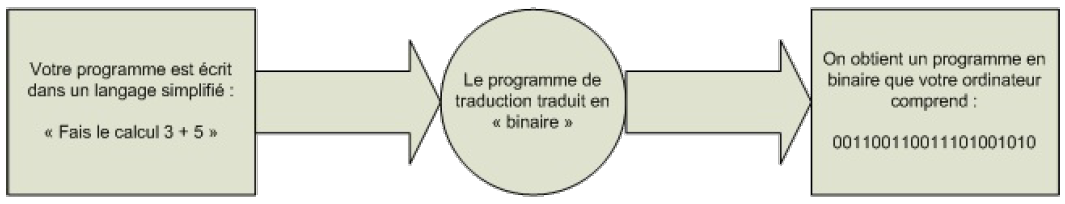
\includegraphics[width=0.9\textwidth]{compilation.png}
  \caption{Le processus de compilation.}
\end{figure}






%----------------------------------------------------
% Section - Qu'est-ce que le Java?
%----------------------------------------------------
%
\section{Qu'est-ce que le Java?}
%
%
Le langage Java a été créé , entre autres, par James Gosling, Patrick Naughton et Mike Sheridan, tous les trois employés chez \emph{Sun Microsystems} dans les années 1990. Sa première version parut en 1995. Java est maintenant propriété de \emph{Oracle Corporation}.

Java est un langage presque entièrement \textbf{orienté objet}. Il reprend une grande partie de la syntaxe du C/C++, tout en y ajoutant certaines fonctionnalités : une librairie standard très complète, la réflexivité, les expressions lambdas, l'\emph{autoboxing} et l'\emph{unboxing}, les interfaces, et plusieurs autres.  Toutefois, les pointeurs et l'héritage multiple ne sont pas supportés. Ils ajouteraient une trop grande complexité au langage, alors que le but de Java est d'être simple, sécuritaire et robuste.

Le Java compte un nombre impressionnant d'utilisateurs. Une de ses forces est d'ailleurs sa portabilité. Tout programme Java, une fois compilé en \emph{bytecode}, peut fonctionner sur n'importe quelle machine, tant qu'une machine virtuelle Java (JRE, ou \emph{Java Runtime Environment}) y est installée.




%--------------------------------------------------------
% Chapitre - Votre premier programme 
%--------------------------------------------------------
%
\chapter{Votre premier programme}

\textit{Manuel de référence : p. 1 à 22 et 33 à 38.}

%--------------------------------------------------------
% Section - Les environnements de développement intégré 
%--------------------------------------------------------
% 
%
\section{L'IDE Visual Studio Code}
%
Pour programmer, il est préférable d'utiliser un bon environnement de développement (\textbf{IDE}, ou \emph{Integrated Development Environment}). De tels logiciels comprennent un \textbf{éditeur de texte}, un \textbf{compilateur} et un \textbf{débogueur}. Nous utiliserons l'IDE Visual Studio Code\footnote{Pour plus d'informations concernant Visual Studio Code, consultez \href{https://code.visualstudio.com/docs}{code.visualstudio.com/docs}.} avec l'extension WPILib fournie par FIRST.

Visual Studio Code est disponible gratuitement sur \href{https://code.visualstudio.com/}{code.visualstudio.com/}. Vous devrez également vous assurer d'avoir installé une version récente du \href{http://www.oracle.com/technetwork/java/javase/downloads/index.html}{JDK 8} (\emph{Java Development Kit}). Les étapes d'installation sont également détaillées \href{http://wpilib.screenstepslive.com/s/currentCS/m/79833/l/932382-installing-vs-code}{ici}.

% Image - Interface principale de VS Code
%
\begin{figure}[!htb]
  \centering
  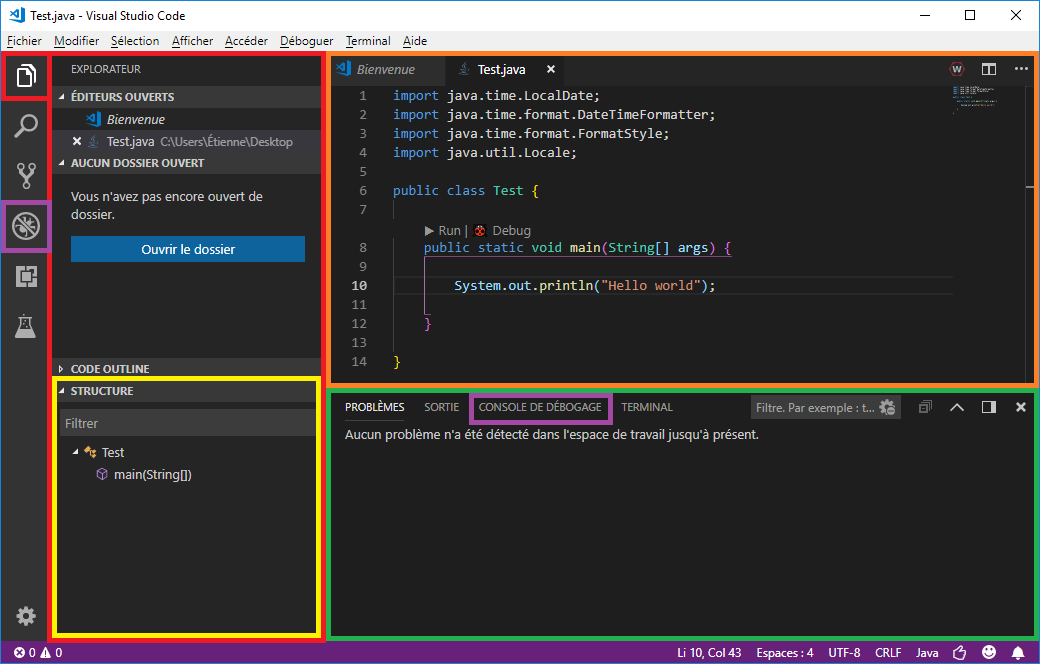
\includegraphics[width=\textwidth]{vs-code-interface.png}
  \caption{L'interface principale de Visual Studio Code.}
\end{figure}
%
Visual Studio Code est un logiciel ayant plusieurs fonctionnalités. On peut d'ailleurs lui en ajouter à l'aide d'extensions (\emph{plugins}), comme celle que nous utiliserons pour développer sur le roboRIO. Voici les sections qui nous intéresseront le plus :

\begin{labeling}{\ Package Explorer\ }
%
\item[\colorbox{ec-red}{Explorateur}] Cette fenêtre regroupe les fichiers de votre projet, subdivisés en dossiers et paquetages (\emph{packages}), jusqu'aux fichiers Java.
%
\item[\colorbox{ec-orange}{Fenêtre d'édition}] Cette fenêtre affiche tous les fichiers que vous êtes en train d'éditer, vous permettant facilement de naviguer entre différents documents.
%
\item[\colorbox{ec-yellow}{Structure}] Cette section affiche la structure du fichier en cours d'édition.
%
\item[\colorbox{ec-green}{Problèmes}] Comme son nom l'indique, on y retrouve une liste de tous les avertissements et erreurs concernant votre projet. Chaque item précise la nature de l'erreur et où elle se trouve.
%
\item[\colorbox{ec-purple}{Débogage}] La console est un outil essentiel, c'est le premier lien entre vous et l'exécution de votre programme. Vous pourrez y afficher du texte et en insérer.
\end{labeling}

L'interface est personnalisable, à vous de l'adapter comme il vous plaira!






%--------------------------------------------------------
% Section - Création du projet 
%--------------------------------------------------------
%
\section{Création d'un programme Java}
%
\begin{enumerate}
\item Créez un dossier vide qui contiendra votre projet.
\item Faites un clic droit sur votre dossier, puis sélectionnez \commande{Open with Code}. Vous pouvez aussi choisir \commande{Fichier > Ouvrir le dossier...}, directement dans VS Code. 
\item Dans VS Code, créez un nouveau fichier avec \commande{Fichier > Nouveau fichier}. Un fichier vide sera créé.

\item \begin{minipage}[t]{\linewidth}
          %\raggedright
          \begin{center}
          \adjustbox{valign=t}{%
            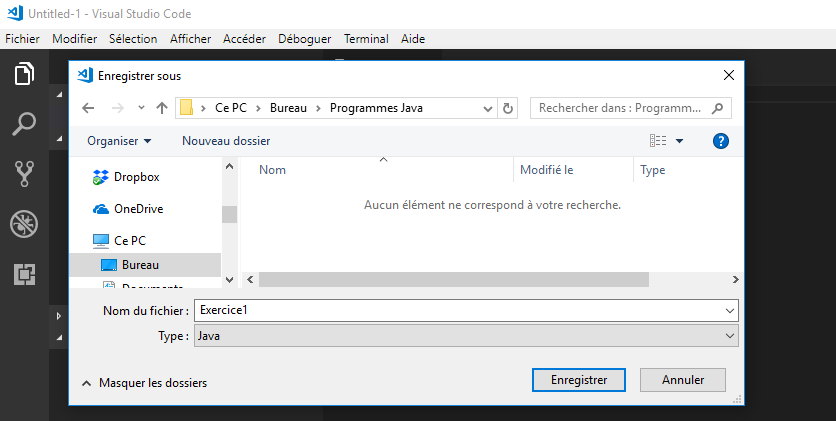
\includegraphics[width=.9\linewidth]{vs-code-save.png}%
          }
          \end{center}
          
          \medskip
          Enregistrez votre fichier dans le même dossier avec \commande{Fichier > Enregistrer sous...}, ou \commande{Ctrl + S}. Donnez un nom à votre programme (sans espace débutant par une majuscule) et sélectionnez \commande{Java} comme type de fichier. Cliquez sur \commande{Enregister}.
       \end{minipage}

\item Complétez votre fichier avec l'exemple suivant.
\end{enumerate}
%
% Code - Programme de base
%
\begin{MyTCB}{Programme de base}
public class Exercice1 {

	public static void main(String[] args) {
	
		System.out.println("Hello, world");
		
	}
	
}
\end{MyTCB}
%
%
% Image - Compiler/Exécuter avec VS Code
\begin{figure}[H]
	\centering
	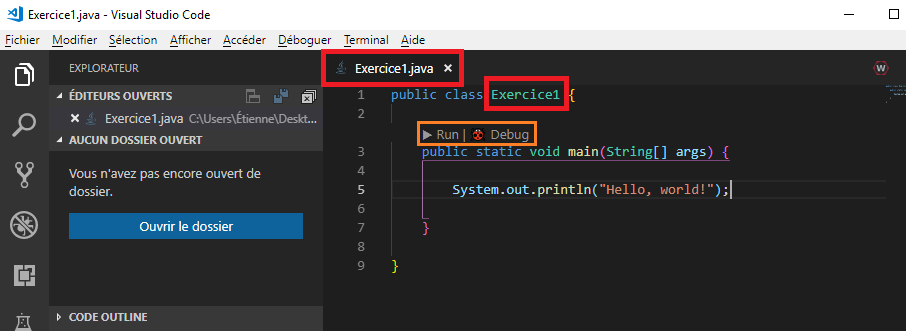
\includegraphics[width=\textwidth]{vs-code-premier-programme.png}
	\caption{Compiler, exécuter et déboguer un programme avec VS Code.}
\end{figure}
%
Attention! Il est très important que le \colorbox{ec-red}{nom de votre classe} (à côté du mot \texttt{class}) soit le même que le \colorbox{ec-red}{nom de votre fichier} (par exemple, \textit{Exercice1}).

En \colorbox{ec-orange}{orange}, le bouton \commande{Run} vous permet de compiler et d'exécuter votre programme, tandis que \commande{Debug} lance votre programme en mode débogage. En appuyant sur l'un ou l'autre, vous devriez voir du texte apparaître dans votre console.
%
% Image - Écriture console
%
\begin{figure}[!ht]
	\centering
	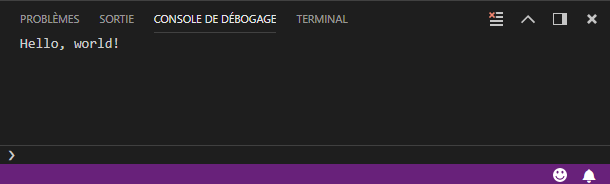
\includegraphics[scale=1]{vs-code-console.png}
	\caption{Écriture dans la console.}
\end{figure}

Si la console n'est pas déjà affichée, il suffit de cliquer sur \commande{Afficher > Console de débogage}, ou \commande{Ctrl + Shift + Y}.

Il est également possible d'ouvrir automatiquement la console lorsque vous démarrez un programme. Cliquez sur \commande{Fichier > Préférences > Paramètres}, ou \commande{Ctrl + ,}. Dans la barre de recherche, saisissez \commande{open console}. À l'option \textit{Contrôle le moment où la console de débogage interne doit s’ouvrir}, choisissez \commande{openOnSessionStart}.

Félicitations, vous venez d'exécuter votre premier programme! Analysons en détail ce qu'il se passe à l'intérieur.






%--------------------------------------------------------
% Section - Instructions
%--------------------------------------------------------
%
\section{Les instructions}
En Java, une \textbf{instruction} est une commande effectuant une certaine action. On écrit une instruction par ligne, et chacune se termine toujours par un \textbf{point-virgule} (\ {;}\ ). Pour l'instant, votre programme ne contient qu'une instruction : 
\begin{code}
System.out.println("Hello, world!");
\end{code}
Vos instructions sont écrites dans la méthode \texttt{\bfseries main}. En Java, tous les programmes ont une méthode \texttt{main}. Il s'agit, en quelque sorte, du point d'entrée du programme.





%--------------------------------------------------------
% Section - Les chaînes de caractères
%--------------------------------------------------------
%
\section{Les chaînes de caractères}
%
Le rôle de votre programme est d'afficher du texte dans la console. Vous avez sûrement remarqué que le texte à afficher est encadré de guillemets anglais ("..."), mais qu'ils n'apparaissent pas dans la console. Ils sont essentiels pour que le compilateur fasse la différence entre du code et du texte. On les appelle des \textbf{chaînes de caractères}, ou \emph{\bfseries String} en anglais. Essayer de modifier le texte entre les guillemets et d'exécuter votre programme : vous constaterez que la chaîne de caractères affichée dans la console s'est modifiée!

On peut joindre plusieurs chaînes de caractères avec l'opérateur \commande{+}. Cette opération s'appelle la \textbf{concaténation}. On peut donc écrire :%
\begin{code}
System.out.println("Bonjour " + "à tous" + " et à toutes" + "!");
\end{code} 





%--------------------------------------------------------
% Section - La méthode println
%--------------------------------------------------------
%
\section{La méthode \texttt{println()}}
%
En Java, une \textbf{méthode} est une instruction qui réalise une opération prédéfinie. On utilise une méthode en écrivant son nom suivi d'une paire de parenthèses. Certaines méthodes ont besoin de paramètres pour effectuer leur travail. C'est le cas de la méthode \texttt{System.out.println()}, qui demande un \emph{String} en paramètre. Elle s'occupe ensuite de l'afficher sur la console.




%--------------------------------------------------------
% Section - Indentation
%--------------------------------------------------------
%
\section{L'indentation}
%
Dans l'exemple précédent, vous pouvez constater qu'à chaque fois que des accolades (\{...\}) sont ouvertes, on ajoute de l'espace au code qui se situe à l'intérieur. C'est ce que l'on appelle l'\textbf{indentation} du code. C'est essentiel pour rendre le code clair et facile à modifier. Pour indenter son code, on ajoute une tabulation (touche \commande{Tab $\rightleftarrows$}) pour chaque paire ouverte d'accolades. VS Code s'en occupe automatiquement la plupart du temps. Dans votre fichier, vous pouvez également faire \commande{Clic droit > Mettre en forme le document} pour corriger l'espacement et l'indentation.







%--------------------------------------------------------
% Section - Les commentaires
%--------------------------------------------------------
%
\section{Les commentaires}
%
%
%
\subsection{Les commentaires standards}
%
%
Lors de l'écriture, il est possible de spécifier au compilateur de ne pas compiler certaines parties du code. C'est ce qu'on appelle les \textbf{commentaires}. Ils permettent de spécifier l'utilité des variables, des méthodes, des classes, etc. Il est crucial d'en ajouter, surtout lors d'un projet en collaboration avec plusieurs personnes!

%
% Code - Premier programme avec commentaires standards
%
\begin{MyTCB}{Programme de base avec commentaires}
/* 
 * La classe suivante affiche un message
 * dans la console.
 */
public class MonPremierProgramme {

	/*  Fonction principale
		du programme.		*/
	public static void main(String[] args) {
	
		//Début du programme
		
		System.out.println("Hello, world"); //Affichage du message
		
	}
	
}
\end{MyTCB}
%
%
Les plus courants sont les \textbf{commentaires en fin de ligne}. Ils débutent par deux barres obliques \mbox{\commande{//}.} Ils informent le compilateur d'ignorer tout le reste de la ligne. Ils sont souvent courts et précis. On les utilise pour mettre en contexte une instruction ou en début de section.

Pour de longs commentaires, on utilise les \textbf{commentaires en blocs}. Ils débutent par \commande{/*} et se terminent par \commande{*/}. Le compilateur ignore alors tout ce qui se trouve entre ces deux balises, un peu comme des parenthèses. On les utilise, entre autres, en entête de fichier, pour spécifier le rôle du fichier (ou de la classe), les noms des auteurs et les dates de création et de modification.

Il est important de mettre des commentaires, mais il ne faut pas en abuser (comme dans l'exemple précédent). Il suffit de trouver le juste équilibre entre clarté et concision. Il est également essentiel de mettre en contexte l'instruction.

Bon commentaire :
\begin{code}
age += 1; // L'utilisateur vieillit d'un an.
\end{code}

Mauvais commentaire :
\begin{code}
age += 1; // Ajout de 1 à la variable age.
\end{code}


% Commentaires Javadoc
%
\subsection{Les commentaires Javadoc}
%
%
Ces commentaires spéciaux sont propres au Java. Ils permettent de créer une documentation accessible pour votre projet. Ils sont très semblables aux commentaires en blocs : il suffit de les faire débuter avec deux étoiles \commande{/**}. Vous aurez donc accès au contenu de votre commentaire partout dans votre projet, sans devoir ouvrir à nouveau le fichier d'origine! 

Pour afficher la Javadoc d'un élément, il suffit de laisser son curseur au-dessus de lui pendant quelques instants.
%
% Code : Commentaire Javadoc
%
\begin{MyTCB}{Ajout de commentaires Javadoc}
/**
 * Ceci est un commentaire Javadoc!
 * @author Etienne
 *
 */
public class MonPremierProgramme { ... }
\end{MyTCB}
%
%
\begin{figure}[!ht]
	\centering
	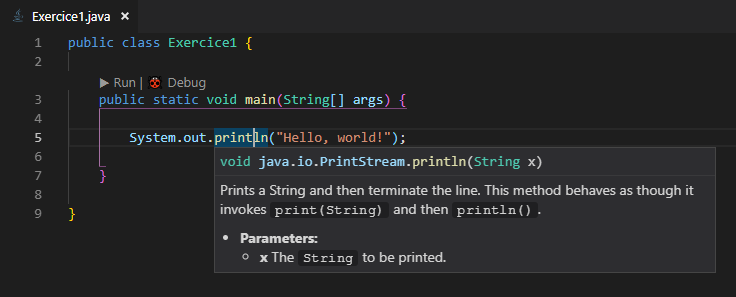
\includegraphics[width=0.99\linewidth]{vs-code-javadoc.png}
	\caption{Visualisation de la Javadoc dans VS Code}
\end{figure}
%
%
La Javadoc possède plusieurs attributs spéciaux débutant par une arrobe \commande{@}. Les exemples de ce guide feront appel aux trois attributs suivants.

\begin{labeling}{@author\ }

\item[\textbf{@author}] On l'utilise dans l'entête d'une classe pour en spécifier l'auteur.
\item[\textbf{@param}] Dans l'entête de méthodes, il précise le rôle de chaque paramètre.
\item[\textbf{@return}] Également dans l'entête de méthodes, il précise la valeur de retour.

\end{labeling}
%


\section{Afficher les caractères internationaux dans VS Code}

\begin{itemize}
	\item Cliquez sur \commande{Fichier > Préférences > Paramètres}, ou \commande{Ctrl + ,}.
	\item Dans la barre de recherche, saisissez \commande{vmargs}, puis cliquez sur \commande{Modifier dans settings.json} du premier résultat.
	\item Cliquez sur le crayon pour modifier la propriété sélectionnée, puis sur \\ 	\commande{Remplacer dans les paramètres}.
	\item À la fin de la chaîne de caractères sélectionnée, ajoutez \commande{\texttt{-Dfile.encoding=UTF-8}}.
	\item Sauvegardez avec \commande{Ctrl + S}.
	\item Lorsque VS Code vous propose de redémarrer, sélectionnez \commande{Restart now}.
\end{itemize}

\begin{figure}[H]
\centering
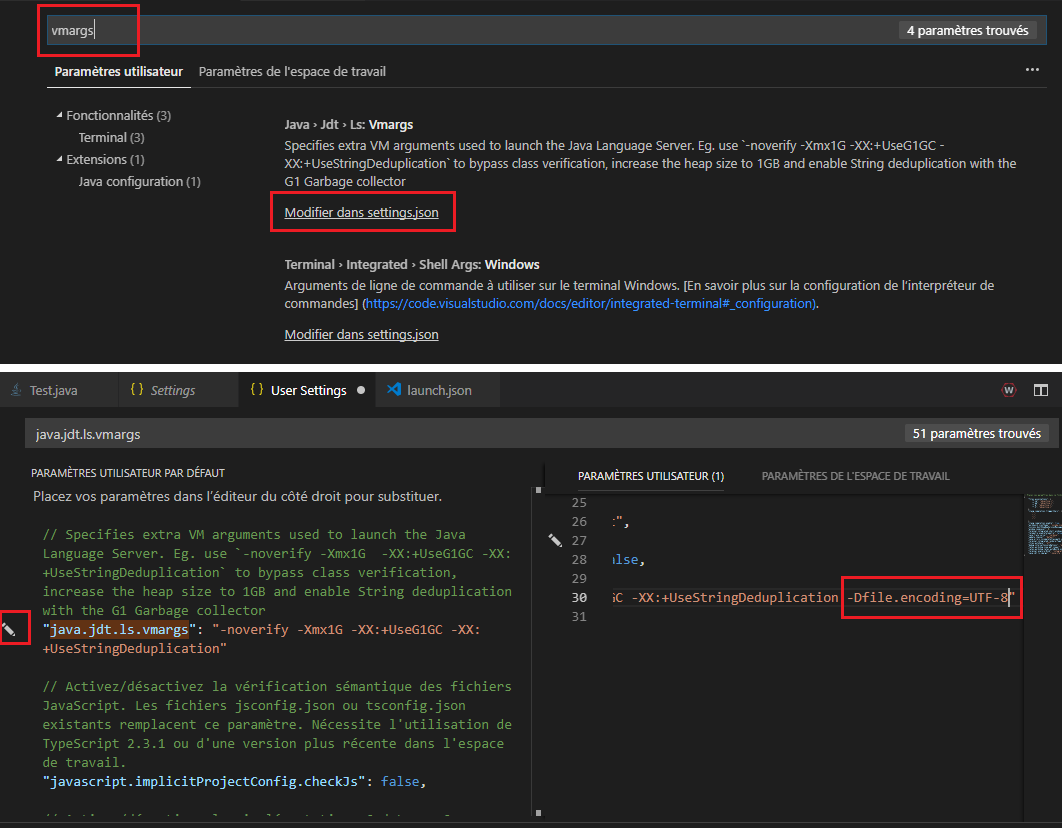
\includegraphics[width=0.99\linewidth]{vscode-file-encoding.png}
\caption{Afficher des caractères internationaux dans la console avec VS Code.}
\end{figure}


%----------------------------------------------------
%
%
% Chapitre 3 - Variables et opérateurs
%
%
%----------------------------------------------------
\chapter{Variables et opérateurs}

\textit{Manuel de référence : p. 23 à 32.}

%--------------------------------------------------------
% Section - Déclaration
%--------------------------------------------------------
%
\section{La déclaration de variables}
%
Une \textbf{variable} est une case mémoire pouvant contenir un certain type de données. Comme son nom l'indique, sa valeur est \emph{variable} : elle peut changer au cours de l'exécution.

\begin{figure}[!ht]
	\centering
	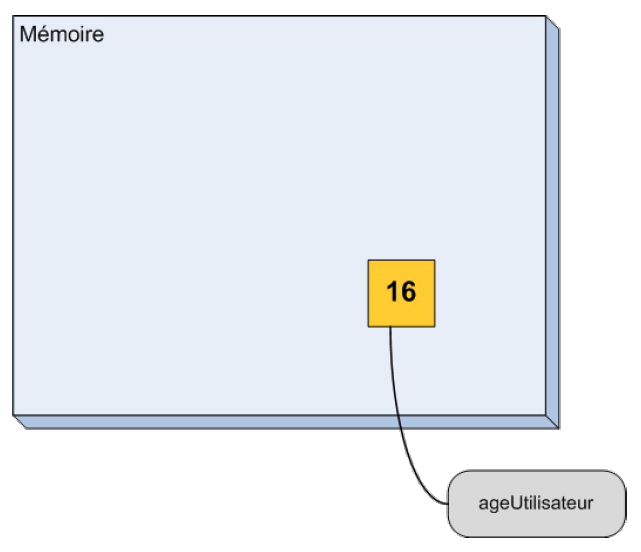
\includegraphics[scale=0.75]{variable-memoire.png}
	\caption{Une variable contenant l'âge de l'utilisateur en mémoire.}
\end{figure}

Pour commencer, regardons un programme utilisant une variable de type \emph{String}.

\begin{MyTCB}{Utilisation d'une variable String}
/**
 * Affiche des noms dans la console.
 * 
 * @author Etienne
 */
public class AffichageNom {

	public static void main(String[] args) {
		
		String nom = "Étienne"; // Nom de l'utilisateur
		
		System.out.println("Je m'appelle " + nom + "!"); // Affichage
		
		nom = "Alexandre"; // Nouvelle valeur
		
		System.out.println("Je m'appelle maintenant " + nom + "!"); // Affichage de la nouvelle valeur
		
	}

}
\end{MyTCB}

\begin{tcolorbox}[title={Sortie console}, sharp corners = south, boxsep = 1.5mm] \tt
	Je m'appelle Étienne!\\
	Je m'appelle maintenant Alexandre!
\end{tcolorbox}

On commence par créer la variable \texttt{nom} de type \emph{String} et on lui donne la valeur \texttt{"Étienne"}. Pour mettre une valeur dans une variable, on utilise le signe égal \commande{=}. L'affectation se fait toujours \textbf{de la droite vers la gauche ($\boldsymbol{\Leftarrow}$)}. On affiche ensuite la valeur de \texttt{nom} dans la console. À la troisième instruction, on met la valeur \texttt{"Alexandre"} dans \texttt{nom}. L'ancienne valeur est alors \textbf{écrasée} par la nouvelle. La dernière instruction affiche la nouvelle valeur de \texttt{nom} dans la console.


% Déclaration de variables
%
\begin{tcolorbox}[enhanced,colframe=ultRed,
	title={Déclaration et initialisation de variables},
	sharp corners=south,
	boxsep = 1.5mm]
Déclaration et initialisation ($\Leftarrow$) dans la même instruction\\
\texttt{\color{ultRed} type} \texttt{\color[RGB]{255, 34, 12} nomVariable} = \texttt{\color[RGB]{63, 136, 197} valeur};%
%
\tcblower
%
Déclaration, puis affectation ($\Leftarrow$) d'une valeur  plus tard dans le programme\\
\texttt{\color{ultRed} type} \texttt{\color[RGB]{255, 34, 12} nomVariable};\\
...\\
\texttt{\color[RGB]{255, 34, 12} nomVariable} = \texttt{\color[RGB]{63, 136, 197} valeur};
\end{tcolorbox}


Lorsque c'est possible, on déclare et on initialise une variable en même temps. C'est ce qui a été fait dans l'exemple précédent. Lorsqu'on ne connaît pas quelle valeur lui donner, on peut la déclarer et lui donner une valeur plus tard.

On peut donner n'importe quel nom à une variable, tant qu'il respecte les conditions suivantes :
\begin{itemize}
	\item pas d'espace ni d'accent;
	\item ne commence pas par un chiffre;
	\item commence par une minuscule;
	\item si son nom est composé de plusieurs mots, les autres mots peuvent commencer par une majuscule.
\end{itemize}

Par exemple, les identificateurs \texttt{prix}, \texttt{ageUtilisateur}, \texttt{vitessexGauche1} et \texttt{estOuvert} respectent cette convention. 




%--------------------------------------------------------
% Section - Lire console
%--------------------------------------------------------
%
\section{Lire la console}
%
Vous savez déjà comment afficher du texte dans la console avec la méthode \texttt{System.out.println()}. Par contre, il pourrait être pratique de lire ce qui est écrit dans la console. Pour effectuer cette tâche, nous utiliserons la class \texttt{Scanner} de la manière suivante.

\begin{figure}[H]
\centering
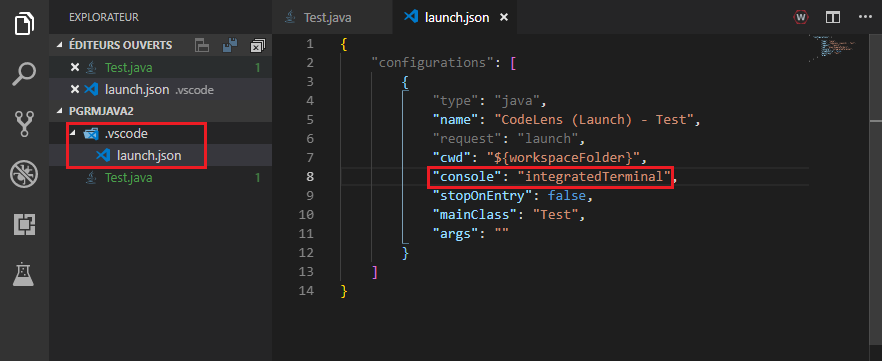
\includegraphics[width=0.99\linewidth]{vscode-integrated-terminal.png}
\caption{Configuration nécessaire pour lire la console dans VS Code.}
\end{figure}

% Code Scanner
%
\begin{MyTCB}{Demander et afficher un nom}
import java.util.Scanner;

/**
 * Demande le nom de l'utilisateur, puis l'affiche.
 * 
 * @author Etienne
 */
public class DemanderNom {

	public static void main(String[] args) {
		
		String nom;
		Scanner scanner = new Scanner(System.in);
		
		//Demander le nom
		System.out.print("Saisissez votre nom : ");
		nom = scanner.nextLine();
		
		//Affichage
		System.out.println("Votre nom est " + nom + "!");

	}

}
\end{MyTCB}

\begin{console}
Saisissez votre nom : {\color{blue} Étienne}\\
Votre nom est Étienne!
\end{console}
Ici, on déclare une variable sans l'initialiser. C'est tout à fait logique, car on ne connaît pas encore le nom à afficher. On déclare ensuite une variable spéciale : la variable \texttt{scanner} de type \texttt{Scanner}. C'est elle qui va nous permettre de lire les entrées dans la console. Remarquez son initialisation : on utilise le \commande{new} suivi de \texttt{Scanner}, le type de notre variable. Nous verrons plus loin que c'est parce que \commande{scanner} est un \textbf{objet}, une sorte de « super-variable ». 

Par la suite, on utilise une variante de \texttt{println()} : la méthode \texttt{print()}. Elles agissent presque de la même façon, sauf que \texttt{print()} n'ajoute pas de saut de ligne après avoir affiché le texte. Essayez les deux et constatez la différence.

Ensuite, on utilise notre \texttt{scanner} et on appelle sa méthode \texttt{nextLine()}. Cela indique au programme de faire une pause jusqu'à ce qu'on écrive un mot dans la console et qu'on appuie sur la touche \commande{Entrée}. Le texte saisi est ensuite stocké dans la variable \texttt{nom} grâce à l'opérateur \commande{=}.

Finalement, on affiche la valeur de \texttt{nom} par concaténation avec d'autres chaînes de caractères. 


%--------------------------------------------------------
% Section - Types primitifs
%--------------------------------------------------------
%
\section{Les variables de type primitif}
%
Jusqu'à présent, nous avons uniquement déclaré des variables de type \texttt{String} et \texttt{Scanner}. Ces variables sont en vérité des \textbf{objets}. Nous verrons plus tard ce que cela signifie. Il existe cependant des types de variables qui sont à la base de tout : les types primitifs. 

\begin{center}
	\renewcommand{\arraystretch}{1.5}
	\begin{tabular*}{\linewidth}{@{\extracolsep{\fill} } l l l} \toprule
		\textbf{Type} & \textbf{Ce qu'il contient} & \textbf{Exemple} \\ \midrule
		\texttt{int} & Un nombre entier. & \texttt{int ageUtilisateur = 20;} \\
		\texttt{double} & Un nombre à virgules de précision double. & \texttt{double prix = 19.95;} \\
		\texttt{boolean} & Une valeur booléenne (\textbf{true} ou \textbf{false}). & \texttt{boolean estOuvert = true;} \\ \bottomrule
	\end{tabular*}
	\captionof{figure}{Les types primitifs les plus utilisés.}
\end{center}

Ces types débutent par une minuscule puisqu'ils sont primitifs, alors que \texttt{String} et \texttt{Scanner} débutent par une majuscule puisqu'ils représentent une classe d'objets. 

\begin{MyTCB}{Affichage de variables primitives}
/**
 * Affiche des données de type primitif.
 * 
 * @author Etienne
 */
public class AffichagePrimitif {

	public static void main(String[] args) {
		
		int age = 14, ageAmi = 13;
		double taille = 1.45;
		
		System.out.println("J'ai " + age + " ans!");
		System.out.println("Mon ami a " + ageAmi + " ans.");
		System.out.println("Je mesure " + taille + " m.");

	}

}
\end{MyTCB}

\begin{tcolorbox}[title={Sortie console}, sharp corners = south, boxsep = 1.5mm] \tt
	J'ai 14 ans!\\
	Mon ami a 13 ans.\\
	Je mesure 1.45 m.
\end{tcolorbox}

À la ligne 10, on déclare deux variables du même type sur la même ligne. C'est tout à fait légal, il suffit de séparer leurs noms par des virgules.

Avant un \texttt{Scanner}, il est également possible d'obtenir des données de type primitif à partir de la console.

\begin{MyTCB}{Demande de l'âge et de la taille}
import java.util.Scanner;

/**
 * Demande l'âge et la taille de l'utilisateur,
 * puis l'affiche dans la console.
 * 
 * @author Etienne
 */
public class AgeTaille {

	public static void main(String[] args) {
		
		int age;
		double taille;
		Scanner scanner = new Scanner(System.in);
		
		//Demande de l'âge
		System.out.print("Saisissez votre âge : ");
		age = scanner.nextInt();
		
		//Demande de la taille
		System.out.print("Saisissez votre taille : ");
		taille = scanner.nextDouble();
		
		//Affichage
		System.out.println("Vous avez " + age + " ans et mesurez " + taille + " m.");

	}

}
\end{MyTCB}
\begin{console}
	Saisissez votre âge : {\color{blue} 20}\\
	Saisissez votre taille : {\color{blue} 1,80} \\
	Vous avez 20 ans et mesurez 1.8 m.
\end{console}

Tout comme \texttt{nextLine()}, les méthodes \texttt{nextInt()} et \texttt{nextDouble()} attendent qu'une valeur soit saisie dans la console. Elles retournent ensuite ces valeurs pour qu'elles puissent être stockées dans des variables de notre choix.


\section{Les constantes}

Jusqu'à présent, une variable agit comme une case dans laquelle on range une donnée pour pouvoir y faire référence plus tard. Cette valeur peut changer au cours du programme. Cependant, dans certains cas, on peut vouloir que le contenu d'une variable ne puisse pas changer. C'est ce qu'on appelle une \textbf{constante}.

% Déclaration de constantes
%
\begin{tcolorbox}[enhanced,colframe=ultRed,
	title={Déclaration de constantes},
	sharp corners=south,
	boxsep = 1.5mm]
Utilisation du mot-clé \textbf{final}\\
\texttt{final {\color{ultRed}type}} \texttt{\color[RGB]{255, 34, 12} NOM{\_}CONSTANTE} = \texttt{\color[RGB]{63, 136, 197} valeur};%
\end{tcolorbox}

Il suffit d'ajouter le mot-clé \texttt{final} devant la déclaration pour transformer une variable en constante. Il est alors impossible de redéfinir sa valeur. Par convention, le nom d'une constante est écrit tout en majuscules. On utilise alors la barre de soulignement pour séparer les différents mots.

\begin{code}
	final double NOMBRE_NIVEAUX = 10; //Constante
NOMBRE_NIVEAUX = 12; // Le compilateur affiche une erreur!
\end{code}

Les constantes sont très utiles pour les valeurs qui changent rarement et qui sont utilisées à plusieurs endroits. Si cette valeur doit être modifiée, il suffit alors de la changer à un endroit et le tour est joué!



\section{Les opérateurs arithmétiques}

Maintenant que l'on peut stocker des nombres dans des variables, voyons comment effectuer des opérations arithmétiques sur ceux-ci. La priorité des opérations s'applique.

\begin{center}
\begin{tabularx}{0.5\linewidth}{X c} \toprule
\textbf{Opération} & \textbf{Symbole} \\ \midrule
Addition & + \\
Soustraction & - \\
Multiplication & * \\
Division & / \\
Modulo {\footnotesize (reste de la division)} & \% \\ \bottomrule
\end{tabularx}
\captionof{figure}{Les opérateurs arithmétiques.}
\end{center}

\begin{MyTCB}{Années avant la majorité}
import java.util.Scanner;

/**
 * Demande l'âge de l'utilisateur et affiche le nombre
 * d'années avant qu'il soit majeur.
 * 
 * @author Etienne
 */
public class Majorite {

	public static void main(String[] args) {
		
		int age;
		final int AGE_MAJORITE = 18; // L'âge de la majorité est fixe
		Scanner scanner = new Scanner(System.in);
		
		//Demander l'âge
		System.out.print("Saisissez votre âge : ");
		age = scanner.nextInt();
		
		//Âge avant majorité
		System.out.println("Vous serez majeur dans " + (AGE_MAJORITE - age) + " ans.");

	}

}
\end{MyTCB}
\newpage

\begin{MyTCB}[breakable]{Liquidation d'un inventaire}
import java.util.Scanner;

/**
 * Gestion de la liquidation
 * d'un inventaire.
 * 
 * @author Etienne
 */
public class Liquidation {

	public static void main(String[] args) {
		
		int joursRestants; // Nombre de jours avant la fermeture
		
		int nombreItems; // Nombre d'items restants en inventaire
		double prixItem; // Prix d'un item
		double prixTotal; // Prix d'un item avec les taxes
		double valeurInventaire; // Valeur de tous les items
		
		final double TAXES = 1.15; // Taxes fixes de 15%
		
		Scanner scanner = new Scanner(System.in);
		
		
		// Nombre de jours restants
		System.out.print("Nombre de jours avant la fermeture : ");
		joursRestants = scanner.nextInt();
		
		// Nombre d'items
		System.out.print("Nombre d'items restants : ");
		nombreItems = scanner.nextInt();
		
		// Prix d'un item
		System.out.print("Prix d'un item : ");
		prixItem = scanner.nextDouble();
		
		// Prix total d'un item
		prixTotal = prixItem * TAXES;
		
		// Valeur de l'inventaire
		valeurInventaire = prixItem * nombreItems;
		
		// Affichage
		System.out.println("Le prix à payer avec taxes est de " + prixTotal + "$.");
		System.out.println("Votre inventaire vaut " + valeurInventaire + "$.");
		System.out.println("Pour tout liquider, vous devrez vendre environ " + (nombreItems / joursRestants) + " items par jour.");
		
	}
}
\end{MyTCB}
%
\begin{console}
Nombre de jours avant la fermeture : {\color{blue} 10}\\
Nombre d'items restants : {\color{blue} 50}\\
Prix d'un item : {\color{blue} 11,40}\\
Le prix à payer avec taxes est de 13.11\$.\\
Votre inventaire vaut 570.0\$.\\
Pour tout liquider, vous devrez vendre environ 5 items par jour.
\end{console}

Dans les deux exemples précédents, on effectue des calculs avant l'affectation d'une variable ou directement dans un \texttt{println()} pour afficher le résultat. Les deux sont acceptables, tant que le code reste clair et que les parenthèses sont placées aux bons endroits. Dans le cas de calculs longs et compliqués, il est préférable de les isoler pour que ce soit plus lisible.

\section{Les opérateurs d'affectation}
Vous connaissez déjà l'opération d'affectation de base : le symbole égal \commande{=}. C'est le plus commun. Il existe cependant des raccourcis qui peuvent être utiles dans plusieurs cas. Dans tous les cas, l'affectation se fait toujours \textbf{de la droite vers la gauche ($\boldsymbol{\Leftarrow}$)}.

\begin{center}
\renewcommand{\arraystretch}{1.5}
	\begin{tabularx}{\linewidth}{l c X X} \toprule
		\textbf{Rôle} & \textbf{Symbole} & \textbf{Exemple} & \textbf{Équivalent} \\ \midrule
		Ajout de... & \texttt{+=} & \texttt{age += 2;} & \texttt{age = age + 2;} \\
		Retrait de... & \texttt{-=} & \texttt{vie -= dommages;} & \texttt{vie = vie - dommages;} \\
		Multiplier par... & \texttt{*=} & \texttt{prix *= rabais;} & \texttt{prix = prix * rabais;} \\
		Diviser par... & \texttt{/=} & \texttt{taille /= 3.28;} & \texttt{taille = taille / 3.28;} \\
		Incrémentation & \texttt{++} & \texttt{compteur++;} & \texttt{compteur += 1;} \\
		Décrémentation & \texttt{-{}-} & \texttt{points-{}-;} & \texttt{points -= 1;} \\ \bottomrule
	\end{tabularx}
	\captionof{figure}{Les opérateurs d'affectation.}
\end{center}


\section{La librairie \texttt{Math}} \label{lib-math}
Java a une librairie standard très fournie. Elle comprend, entre autres, la classe \texttt{Math}. Celle-ci fournit plusieurs fonctions mathématiques de base : 
\begin{itemize}
	\item la valeur absolue (\texttt{abs}),
	\item les exposants (\texttt{pow}),
	\item les fonctions trigonométriques (\texttt{sin}, \texttt{cos}, \texttt{tan}, etc.),
	\item le maximum et le minimum (\texttt{max} et \texttt{min}),
	\item la racine carrée (\texttt{sqrt}),
	\item l'arrondi (\texttt{round}, \texttt{ceil} et \texttt{floor}).
\end{itemize}

\begin{MyTCB}{Utilisation de la classe Math}
import java.util.Scanner;

/**
 * Affiche la valeur absolue et le cube d'un nombre.
 * 
 * @author Etienne
 *
 */
public class TestMath {

	public static void main(String[] args) {
		
		double nombre;
		Scanner scanner = new Scanner(System.in);
		
		//Obtention du nombre
		System.out.print("Saisissez un nombre : ");
		nombre = scanner.nextDouble();
		
		//Calculs
		System.out.println("\nLa valeur absolue du nombre est : " + Math.abs(nombre));
		System.out.println("Le cube du nombre est : " + Math.pow(nombre, 3));

	}

}
\end{MyTCB}

La méthode \texttt{pow()} prend deux paramètres : le premier est la base et le deuxième est l'exposant. Ainsi, \texttt{pow(x, y)} $= x^y$.




%----------------------------------------------------
%
%
% Chapitre 4 - Instructions conditionnelles
%
%
%----------------------------------------------------
\chapter{Les instructions conditionnelles}

\textit{Manuel de référence : p. 39 à 46.}

\section{Le \textit{if else}}
Jusqu'à présent, vos programmes se sont exécutés de manière \textbf{séquentielle} : toutes les instructions sont exécutées les unes après les autres. En réalité, il est bien rare qu'un programme suive une seule séquence. Avec les \textbf{instructions conditionnelles}, il sera possible d'exécuter une certaine partie de votre programme uniquement si une certaine condition est respectée. Nous utiliserons alors le \emph{if else}.

\begin{tcolorbox}[enhanced,colframe=ultRed,
	title={La structure \emph{if else}},
	sharp corners=south,
	boxsep = 1.5mm]
\texttt{{\color{ultRed}if} (} {\color[RGB]{255, 34, 12} condition} \texttt{) \{}\\
	\hspace*{0.5cm} {\color[RGB]{63, 136, 197} instruction1};\\	
	\hspace*{0.5cm} ... \texttt{// Si la condition est vraie...}\\
\texttt{\}\\
{\color{ultRed} else} \{ // Facultatif \\}
	\hspace*{0.5cm} {\color[RGB]{63, 136, 197} instruction2};\\ 
	\hspace*{0.5cm} ... \texttt{// Si la condition est fausse...} \\
\texttt{\}}
%
\end{tcolorbox}

Si la condition donnée est vraie, alors les instructions contenues dans le premier bloc seront exécutées. Sinon, ce sont celles du deuxième bloc qui seront exécutées. Le \emph{else} est facultatif. S'il n'y a pas de \emph{else} et que la condition est fausse, alors le programme continue son exécution normalement, sans exécuter le contenu du \emph{if}.

Comme une condition peut être vraie ou fausse, on dit que c'est une condition \textbf{booléenne}. C'est d'ailleurs une des principales utilités du type \texttt{boolean}.



\section{Les opérateurs de comparaison et les opérateurs logiques}

Pour exprimer une condition, on peut utiliser les \textbf{opérateurs de comparaison} et les \textbf{opérateurs logiques}. Les principaux sont les suivants.

\begin{center}
\renewcommand{\arraystretch}{1.5}
	\begin{tabularx}{0.8\linewidth}{l c X X} \toprule
		\textbf{Rôle} & \textbf{Symbole} & \textbf{Exemple} \\ \midrule
		égal & \texttt{==} & \texttt{a == 2} \\
		n'est pas égal & \texttt{!=} & \texttt{prix != 10} \\
		est plus grand & \texttt{>} & \texttt{rabais > prix} \\
		est plus grand ou égal & \texttt{>=} & \texttt{age >= AGE\_MAJORITE} \\
		est plus petit & \texttt{<} & \texttt{rotation < 25.1} \\
		est plus petit ou égal & \texttt{<=} & \texttt{distance <= 120} \\
		ou & \texttt{||} & \texttt{a == 10 || b == 5} \\
		et & \texttt{\&\&} & \texttt{distance >= 10 \&\& angle == 180} \\
		n'est pas & \texttt{!} & \texttt{!estOuvert} \\ \bottomrule
	\end{tabularx}
	\captionof{figure}{Les opérateurs de comparaison et les opérateurs logiques.}
\end{center}

Les six premiers sont appelés les \textbf{opérateurs de comparaison}. On les utilise pour comparer des nombres ensemble. Les trois derniers sont appelés les \textbf{opérateurs logiques}. Ils permettent de modifier d'autres conditions ou booléens. Avec le \textbf{ou}, la nouvelle condition est vraie si la première ou la deuxième condition est vraie. Quant au \textbf{et}, il faut que les deux conditions soient vraies pour que la nouvelle condition soit vraie. Finalement, le dernier opérateur permet d'inverser une valeur booléenne. 


\begin{MyTCB}{Validation d'une année de naissance}
import java.time.LocalDate;
import java.util.Scanner;
/**
 * Validation d'une année de naissance.
 * 
 * @author Etienne
 */
public class ValidationNaissance {

	public static void main(String[] args) {
		
		int annee;
		final int ANNEE_MINIMALE = 1900;
		final int ANNEE_COURANTE = LocalDate.now().getYear();
		Scanner scanner = new Scanner(System.in);
		
		
		//Obtention de l'année
		System.out.print("Saisissez une année de naissance : ");
		annee = scanner.nextInt();
		
		
		//Validation
		if(annee >= ANNEE_MINIMALE && annee <= ANNEE_COURANTE) {
			System.out.println("Année valide.");
		}
		else {
			System.out.println("L'année " + annee + " est invalide.");
			System.out.println("Vous devez recommencer!");
		}

	}

}
\end{MyTCB}

\section{Les \textit{else if} multiples}

Le \textit{if else} standard permet de gérer deux possibilités en même temps. Dans certains, on voudrait pouvoir gérer plusieurs cas exclusifs entre eux.

Il est possible d'ajouter un \textit{if} immédiatement après un \textit{else}. Il n'y a donc plus de limite au nombre de possibilités!

\begin{MyTCB}{MessageAge.java}
/**
 * Affiche un message selon l'âge de l'utilisateur.
 */
public class MessageAge {

	public static void main(String[] args) {

		final int AGE_PRIMAIRE = 5;
		final int AGE_SECONDAIRE = 12;
		final int AGE_MAJORITE = 18;		
		
		int age;
		
		Scanner scanner = new Scanner(System.in);
		
		// Obtention de l'âge
		System.out.print("Saisissez votre âge : ");
		age = scanner.nextInt();
		
		// Message selon l'âge
		if(age < 0) {
			System.out.println("Âge invalide!");
		}
		else if(age < AGE_PRIMAIRE) {
			System.out.println("Pas encore à l'école!");
		}
		else if(age < AGE_SECONDAIRE) {
			System.out.println("Au primaire!");
		}
		else if(age < AGE_MAJORITE) {
			System.out.println("Au secondaire!");
		}
		else {
			System.out.println("Vous êtes majeur!");
		}
	}
}
\end{MyTCB}

Comme les \textit{else if} sont imbriqués, \textbf{un seul cas} sera exécuté. Les conditions des \textit{if} sont vérifiées dans le même ordre qu'ils ont été écrits. 

Par exemple, dans l'exemple précédent, supposons que l'âge est de 10 ans. Si on les vérifie individuellement, les deux dernières conditions sont vraies (\verb|age < AGE_SECONDAIRE| et \verb|age < AGE_MAJORITE|). Cependant, la première condition vraie est \verb|age < AGE_SECONDAIRE|, c'est donc ce \textit{if} qui sera exécuté.

\begin{figure}[!htbp]
	\centering
	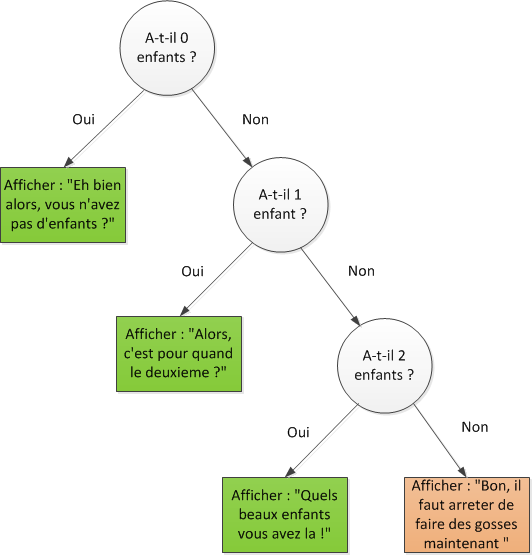
\includegraphics[width=0.6\linewidth]{else-if-multiples.png}
	\caption{La structure des \textit{else if} multiples.}
\end{figure}






\chapter{Les méthodes}

\textit{Manuel de référence : p. 69 à 77}

\section{L'appel de méthodes}

Jusqu'à présent, vous avez utilisé quelques méthodes prédéfinies. Certaines reçoivent des paramètres entre leurs parenthèses, d'autres non. Certaines retournent une valeur, d'autres non. 

En Java, une \textbf{méthode} est une instruction qui réalise une série d'opérations définies ailleurs. On utilise une méthode en écrivant son nom suivi d'une paire de parenthèses. Certaines méthodes ont besoin de paramètres pour effectuer leur travail. C'est le cas de \texttt{println()}, \texttt{nextLine()} et toutes les méthodes de classe \texttt{Math} (voir \ref{lib-math}).

% Utiliser une méthode
%
\begin{tcolorbox}[enhanced,colframe=ultRed,
	title={Utiliser une méthode},
	sharp corners=south,
	boxsep = 1.5mm]
%
Utiliser une méthode sur un objet (instancié avec \texttt{new}) \\[3pt]
\texttt{{\color{ec-green} objet}.{\color[RGB]{255, 34, 12}nomMethode}({\color[RGB]{63, 136, 197}param1}, {\color[RGB]{63, 136, 197}param2}, ...);}\\
\texttt{{\color{ultRed} typeRetour} {\color[RGB]{63, 136, 197}valeurRetournee} = {\color{ec-green} objet}.{\color[RGB]{255, 34, 12}nomMethode}({\color[RGB]{63, 136, 197}param1}, {\color[RGB]{63, 136, 197}param2}, ...);}%
%
\tcblower
%
Utiliser une méthode sur une classe (méthode statique) \\[3pt]
\texttt{{\color{ec-purple} NomClasse}.{\color[RGB]{255, 34, 12}nomMethode}({\color[RGB]{63, 136, 197}param1}, {\color[RGB]{63, 136, 197}param2}, ...);}\\
\texttt{{\color{ultRed} typeRetour} {\color[RGB]{63, 136, 197}valeurRetournee} = {\color{ec-purple} NomClasse}.{\color[RGB]{255, 34, 12}nomMethode}({\color[RGB]{63, 136, 197}param1}, {\color[RGB]{63, 136, 197}param2}, ...);}%
%	
\end{tcolorbox}


\section{Créer une méthode}

\begin{MyTCB}{Programme sans méthode}
public class Bonjour {

    public static void main(String[] args) {

        System.out.println("Bonjour Étienne!");
        System.out.println("Bonjour Camille!");
        System.out.println("Bonjour Alexandre!");
        System.out.println("Bonjour Chaymae!");

    }

}
\end{MyTCB}

Vous aurez sûrement remarqué qu'il vous arrive de réécrire la même opération plusieurs fois. Au lieu de copier-coller ces instructions, vous pouvez déplacer ce bout de code dans une méthode externe, puis l'utiliser comme bon vous semble.

\begin{MyTCB}{Programme avec méthode}
public class Bonjour {

    public static void main(String[] args) {

        direBonjour("Étienne");
        direBonjour("Camille");
        direBonjour("Alexandre");
        direBonjour("Chaymae");
        
    }

    public static void direBonjour(String nom) {
        System.out.println("Bonjour " + nom + "!");
    }

}
\end{MyTCB}

Ainsi, si vous décidez de remplacer \texttt{"Bonjour"} par \texttt{"Bonne journée"}, il vous faudra le remplacer seulement une fois, et non quatre.

\begin{tcolorbox}[enhanced,colframe=ultRed,
	title={Déclarer une méthode},
	sharp corners=south,
	boxsep = 1.5mm]
\texttt{public [static] {\color{ultRed} typeRetour} {\color[RGB]{12, 190, 12} nomMéthode} ({\color[RGB]{63, 136, 197}param1}, {\color[RGB]{63, 136, 197}param2}, ...) \{}\\[2pt]
	\hspace*{0.5cm} \texttt{{\color[RGB]{63, 136, 197} instruction1};}\\
	\hspace*{0.5cm} ... \texttt{// Autres instructions ou calculs}\\
	\hspace*{0.5cm} \texttt{{\color{ultRed}return} {\color[RGB]{255, 34, 12}valeur}; // Facultatif, dépend du type de retour}\\[2pt]
	\texttt{\}}
\end{tcolorbox}

Remarquez que la méthode \texttt{direBonjour} ne retourne aucune valeur. C'est pourquoi son type de retour est \texttt{void}. C'est aussi le cas de la méthode \texttt{println()}.

Des méthodes peuvent, par exemple, effectuer un calcul et retourner un \texttt{double} ou \texttt{int}. D'autres peuvent vérifier une condition et retourner un \texttt{boolean}.

Les méthodes, comme le \texttt{main}, doivent être à l'intérieur d'une classe. Faites attention à bien placer vos accolades.

\begin{code}
// Convertit une durée en secondes
public static int nombreDeSecondes(int heures, int minutes, int secondes) {
	
	int duree = 0;
	
	duree += 60 * 60 * heures;
	duree += 60 * minutes;
	duree += secondes;
	
	return duree;	
	
}
\end{code}

\begin{code}
// Vérifie si une personne est majeure
public static boolean estMajeur(int age) {
	
	return (age >= 18);
	
}
\end{code}


\part{La librairie WPILib}



\chapter{La classe \texttt{TimedRobot}}

\section{Création d'un projet}\label{creationProjetRobot}
Jusqu'à présent, le coeur de vos programmes se trouvait dans la méthode \texttt{main}. Cependant, le comportement d'un robot est plus complexe qu'une simple méthode. Vos prochains programmes auront comme base la classe \texttt{Robot}, héritant de \texttt{TimedRobot}.

\begin{figure}[!htbp]
  \centering
  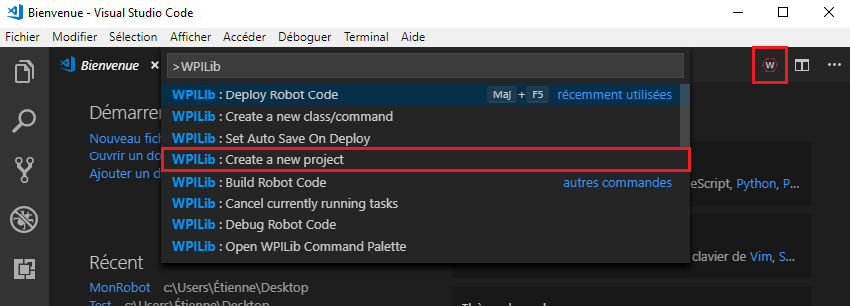
\includegraphics[height=5cm]{vs-code-wpilib.png}
  \caption{Le menu principal de l'extension WPILib.}
\end{figure}

\begin{enumerate}
	\item Dans VS Code, cliquez sur le bouton de l'extension WPILib.
	\item Sélectionnez \commande{WPILib : Create a new project}.
	\item Comme type de projet, sélectionnez \commande{Template}.
	\item Comme langage, sélectionnez \commande{Java}.
	\item Comme projet de base, sélectionnez \commande{Timed Robot}.
	\item Sélectionnez le dossier de sauvegarde de votre projet.
	\item Saisissez le nom de votre projet (sans espace et débutant par une majuscule).
	\item Saisissez le numéro de l'équipe.
	\item Cliquez sur \commande{Generate project}.
\end{enumerate}

Vous vous retrouverez ainsi avec un fichier \commande{Robot.java} contenant le squelette d'un programme pour la FRC.

\section{Les méthodes \texttt{Init} et \texttt{Periodic}}

La classe \texttt{Robot} que VS Code a générée pour vous contient déjà quelques méthodes prédéfinies. Chacune d'entre elles a un rôle bien précis.

\tikzset{>={Stealth[scale=1.3,angle'=45]}}
\begin{figure}[H]
\begin{center}
\begin{tikzpicture}[every node/.style = {shape=rectangle, rounded corners, fill=gray!50, draw, minimum width=3.25cm, minimum height=0.8cm, draw=green!60, fill=green!5, very thick},]

\node (robotInit) at (0,5) {robotInit};
\node (disabledInit) at (0,3) {disabledInit};
\node (disabledPeriodic) at (0,1) {disabledPeriodic};
\node (autonomousInit) at (4.5,3) {autonomousInit};
\node (autonomousPeriodic) at (4.5,1) {autonomousPeriodic};
\node (teleopInit) at (9,3) {teleopInit};
\node (teleopPeriodic) at (9,1) {teleopPeriodic};
\node (testInit) at (13.5,3) {testInit};
\node (testPeriodic) at (13.5,1) {testPeriodic};

\node (periode) [draw=blue!60, fill=blue!5] at (6.75, 5) {Changement de période};

\draw[fill] (0,7) circle [radius=0.25];

\draw[->, to path={-- (\tikztotarget)}] (0,7) edge (robotInit) (robotInit) edge (disabledInit) (disabledInit) edge (disabledPeriodic) (autonomousInit) edge (autonomousPeriodic) (teleopInit) edge (teleopPeriodic) (testInit) edge (testPeriodic);
\draw[->] (-1.0,1.5) arc [radius=0.7, start angle=45, end angle= 315];
\draw[->] (3.25,1.5) arc [radius=0.7, start angle=45, end angle= 315];
\draw[->] (8.0,1.5) arc [radius=0.7, start angle=45, end angle= 315];
\draw[->] (12.5,1.5) arc [radius=0.7, start angle=45, end angle= 315];
\draw (disabledPeriodic) edge ++(0,-1.5) (autonomousPeriodic) edge ++(0,-1.5) (teleopPeriodic) edge ++(0,-1.5) (testPeriodic) edge ++(0,-1.5);
\draw (0,-0.5) -| (16,5);
\draw[->] (16,5) -- (9.1, 5);
\draw (periode) edge (6.75, 4);
\draw[->] (6.75, 4) -| (1.0,3.4);
\draw[->] (6.75, 4) -| (4.5,3.4);
\draw[->] (6.75, 4) -| (9,3.4);
\draw[->] (6.75, 4) -| (13.5,3.4);
\end{tikzpicture}
\caption{Séquence d'exécution des méthodes de la classe Robot.}
\end{center}
\end{figure}

Chaque état dans lequel peut être le robot possède sa méthode \texttt{Init} et \texttt{Periodic}. Par exemple, lorsque le robot entre en période autonome, le contenu de la méthode \texttt{autonomousInit} est appelé une fois. Ensuite, la méthode \texttt{autonomousPeriodic} est appelée en boucle (périodiquement, soit environ aux 20 millisecondes) tant que le robot reste dans cet état.  

La seule exception est la méthode \texttt{robotInit} : elle s'exécute une fois, au tout début, lorsque le programme démarre. Habituellement, on y initialise les différentes composantes du robot, ses sous-systèmes, etc.

\section{Faire avancer le robot}

\begin{MyTCB}{Utilisation de DifferentialDrive avec Joystick}
public class MonPremierRobot extends TimedRobot {
	
	private VictorSP moteurGauche, moteurDroit;
	private DifferentialDrive basePilotable;
	private Joystick joystick;
	
	@Override
	public void robotInit() {
		moteurGauche = new VictorSP(0);
		moteurDroit = new VictorSP(1);
		basePilotable = new DifferentialDrive(moteurGauche, moteurDroit);
		joystick = new Joystick(0);
	}
	
	@Override
	public void autonomousPeriodic() {
		moteurGauche.set(0.5);
		moteurDroit.set(-0.5);
	}
	
	
	@Override
	public void teleopPeriodic() {
		basePilotable.arcadeDrive(-1 * joystick.getY(), joystick.getX());
	}

}

\end{MyTCB}

Dans un premier temps, on déclare comme attributs privés de classe les composantes de notre robot : deux contrôleurs moteur \texttt{VictorSP}, une \text{DifferentialDrive} et un \texttt{Joystick}. On les instancie dans la méthode \texttt{robotInit}.

Ensuite, en période autonome, on met le moteur gauche à 50 \% de sa puissance vers à l'avant, et le moteur droit, à 50 \% vers l'arrière. Le robot tournera donc en rond pendant 15 secondes.

Finalement, en période téléopérée, on utilise la méthode \texttt{arcadeDrive} avec le Joystick pour contrôleur le robot naturellement. 

\subsection{La classe \texttt{VictorSP}}
Cette classe sert à déclarer des contrôleurs moteur de type VictorSP. Des classes existent pour chaque modèle de contrôleur moteur : Talon, Spark, Jaguar, etc.

Son constructeur reçoit en paramètre un nombre entier (voir lignes 9 et 10). Il s'agit du port PWM du RoboRIO où est branché le contrôleur.

Cette classe possède la méthode \texttt{set(double)}. Elle reçoit un nombre compris entre -1.0 et 1.0, spécifiant la puissance à laquelle le moteur doit aller.

\subsection{La classe \texttt{DifferentialDrive}}

Cette classe fournit plusieurs méthodes utiles pour contrôler la base pilotable. Bien qu'il serait possible de calculer manuellement les valeurs à envoyer à chaque moteur, il est plus pratique (et rapide) d'utiliser cette classe. Elle est configurée pour les bases pilotables de type « tank ». Les classes \texttt{MecanumDrive} et \texttt{KilloughDrive} (robot à trois roues) sont également disponibles.

Le constructeur reçoit comme arguments les deux contrôleurs moteur : celui de gauche et celui de droite. La \texttt{DifferentialDrive} doit les avoir en référence pour contrôler la base pilotable.

Sa méthode \texttt{arcadeDrive(double, double)} reçoit deux nombres en paramètre : \texttt{forward} et \texttt{rotation}. Le paramètre \texttt{forward} (entre -1.0 et 1.0) représente la vitesse d'avancée en ligne droite. Le paramètre \texttt{rotation} (entre -1.0 et 1.0) représente la vitesse de rotation, où les valeurs positives vont vers la droite (sens horaire). 

\subsection{La classe \texttt{Joystick}}

On utilise évidemment cette classe pour lire les valeurs d'un Joystick. Son constructeur reçoit en paramètre l'ordre de branchement du Joystick dans la DriverStation (à partir de 0). Cet ordre est très important lorsque le robot est contrôlé par plus d'une manette en même temps.

On accède aux valeurs des axes (de -1.0 à 1.0) avec la méthode \texttt{getRawAxis(int)}, où l'entier en paramètre est le numéro de l'axe (à partir de 0). Des raccourcis existent pour les axes principaux : \texttt{getX()} et \texttt{getY()}. Cependant, l'axe des Y est inversé selon notre logique : il renvoie -1.0 lorsqu'on pousse le Joytick vers l'avant, et 1.0 lorsqu'on le tire vers soi. On multiplie donc cette valeur par -1 avant de l'envoyer comme paramètre \texttt{forward} à \texttt{arcadeDrive} (voir ligne 24).

L'état des boutons est donné par la méthode \texttt{getRawButton(int)}, où l'entier en paramètre est le numéro du bouton (à partir de 1). La méthode renvoie le booléen \texttt{\bfseries true} si le bouton est appuyé, et \texttt{\bfseries false} dans le cas contraire.



\chapter[Les actionneurs]{Les actionneurs \footnote{Référence : \url{http://wpilib.screenstepslive.com/s/currentCS/m/java/c/88897}}}

Plusieurs définissent un robot comme étant une machine qui possède un système logique, des capteurs et des actionneurs. Le système logique, c'est le programme exécuté par le RoboRIO. Les capteurs seront utilisés au prochain chapitre. Quant aux actionneurs (\textit{actuators} en anglais), ce sont toute partie du robot qui crée un mouvement. Plusieurs choix d'actuateurs s'offrent à nous, selon nos besoins.

\section{Les moteurs}
Pour un exemple d'utilisation de moteurs (\texttt{VictorSP}, \texttt{DifferentialDrive}), voir le chapitre précédent.

\section{La pneumatique}
Physiquement, un système pneumatique est composé de plusieurs éléments :

\begin{itemize}
	\item une bonbonne, pour contenir l'air comprimé;
	\item un compresseur, pour comprimer de l'air dans la bonbonne;
	\item un pressostat (\textit{pressure switch} en anglais), pour mesurer la pression dans la bonbonne;
	\item un PCM (module de contrôle pneumatique : \textit{Pneumatic Control Module}), pour activer le compresseur et l'arrêter lorsque la pression est assez élevée;
	\item des vérins (pistons, cylindres pneumatiques), pour effectuer les mouvements désirés;
	\item des solénoïdes, pour laisser passer de l'air dans les vérins.
\end{itemize}

Au niveau de la programmation, les seuls éléments que nous devons gérer sont les solénoïdes. Ceux-ci agissent comme des « portes » qui laissent passer l'air (ou non) selon le signal qu'on leur envoie. Attention : les solénoïdes ne sont pas branchés au RoboRIO, mais bien au PCM.



\subsection{Les solénoïdes simples}

Les solénoïdes simples ne comportent qu'une seule valve. Ils peuvent être dans deux états :

\begin{itemize}
	\item \textbf{false} : la valve est fermée : aucun air n'est envoyé;
	\item \textbf{true} : la valve est ouverte : de l'air est envoyé.
\end{itemize}

Lorsqu'un objet \texttt{Solenoid} est instancié, le PCM active automatiquement le compresseur. Cependant, si le programme ne déclare aucun solénoïde, le compresseur ne s'activera tout simplement pas.

\begin{MyTCB}{Utilisation d'un solénoïde simple}
public class UtilisationSolenoideSimple extends TimedRobot {
	
	private Solenoid solenoid;
	private Joystick joystick;
	
	@Override
	public void robotInit() {
		// Branché sur le port 2 du PCM
		solenoid = new Solenoid(2);
		joystick = new Joystick(0);
	}
	
	@Override
	public void teleopPeriodic() {
	
		if(joystick.getRawButton(1)) {
		
			solenoid.set(true);		
			
		} else {
		
			solenoid.set(false);
			
		}
		
	}

}
\end{MyTCB}

Ce code simple ouvre le solénoïde lorsqu'on appuie sur le bouton 1 du Joystick.



\subsection{Les solénoïdes doubles}

Les solénoïdes doubles comportent deux valves. Ils peuvent donc être dans 3 états différents :

\begin{itemize}
	\item \texttt{\bfseries DoubleSolenoid.Value.kOff} : les deux valves sont fermées : aucun air n'est envoyé;
	\item \texttt{\bfseries DoubleSolenoid.Value.kForward} : la valve avant est ouverte : de l'air est envoyé dans l'avant du vérin.
	\item \texttt{\bfseries DoubleSolenoid.Value.kReverse} : la valve arrière est ouverte : de l'air est envoyé dans l'arrière du vérin.
\end{itemize}

\begin{MyTCB}{Utilisation d'un solénoïde double}

public class UtilisationSolenoideDouble extends TimedRobot {
	
	private DoubleSolenoid solenoid;
	private Joystick joystick;
	
	@Override
	public void robotInit() {
		solenoid = new DoubleSolenoid(3, 4); // Ports 3 et 4 du PCM
		joystick = new Joystick(0);
	}
	
	@Override
	public void teleopPeriodic() {
	
		if(joystick.getRawButton(1))
			solenoid.set(DoubleSolenoid.Value.kForward);		
			
		else if(joystick.getRawButton(2))
			solenoid.set(DoubleSolenoid.Value.kReverse);
			
		else
			solenoid.set(DoubleSolenoid.Value.kOff);

	}

}

\end{MyTCB}

Ce type de solénoïde est particulièrement utile pour ouvrir \textbf{et} fermer rapidement des mécanismes. Par exemple, pour lancer une balle, la séquence suivante pourrait être exécutée :

\begin{enumerate}
	\item le solénoïde double est mis en mode \texttt{kForward} : le vérin s'allonge et éjecte la ballel
	\item une seconde plus tard, le solénoïde est mis en mode \texttt{kReverse} : le vérin se rétracte, prêt à recevoir une autre balle;
	\item une demi-seconde plus tard, le solénoïde est mis en mode \texttt{kOff} : le solénoïde ferme ses valves, se qui permet au compresseur de remplir la bonbonne.
\end{enumerate}

Attention! Il est important de toujours fermer les solénoïdes. Sinon, l'air continue de s'échapper et la bonbonne perd de l'air inutilement.

Dans l'exemple précédent, le constructeur d'un \texttt{DoubleSolenoid} reçoit en paramètres deux entiers, car il est branché à deux ports du PCM. Cela permet de contrôler indépendamment les deux valves du solénoïde.


\section{Les servomoteurs}

Jusqu'à présent, les moteurs que nous avons abordés se contrôlent en terme de puissance : lorsque le programme envoie 0.5 à un VictorSP, celui-ci fonctionnera à 50 \% de sa capacité. Cependant, il peut être intéressant de contrôler la \textbf{position absolue} d'un moteur. C'est pour répondre à ce problème que les servomoteurs ont été créés. Par exemple, on peut fixer une caméra sur un servomoteur pour la faire tourner précisément de 180 degrés et voir derrière le robot.

\begin{MyTCB}{Utilisation d'un servomoteur}

public class UtilisationServo extends TimedRobot {
	
	private Servo servo;
	private Joystick joystick;
	
	@Override
	public void robotInit() {
		servo = Servo(8); // Branché sur le port PWM 8 du RoboRIO
		joystick = new Joystick(0);
	}

	@Override
	public void teleopPeriodic() {
	
		if(joystick.getRawButton(1))
			servo.setAngle(0.0);		
		
		else if(joystick.getRawButton(3))
			solenoid.setAngle(90.0);

	}

}

\end{MyTCB}

Ce programme met le servomoteur à son angle minimum (0.0) au début de la période téléopérée, puis permet de le faire tourner à 3 positions différentes : 0°, 45° et 90°.

La méthode \texttt{setAngle(double)} reçoit en paramètre un nombre entre 0.0 et 180.0, car elle est configurée pour fonctionner avec le servomoteur Hitec HS-322HD, qui a une portée de 180°. Il se peut donc que les valeurs données ne soient pas tout à fait exactes lors de l'utilisation d'autres modèles de servos. Il suffit de faire quelques tests pour déterminer les bons angles.





\chapter[Les capteurs]{Les capteurs \footnote{\url{http://wpilib.screenstepslive.com/s/currentCS/m/java/c/88895}}}

Les capteurs, contrairement aux actionneurs, ne créent aucun mouvement. Ils fournissent au robot des informations sur son environnement et ses déplacements.


\section{Les interrupteurs de fin de course}

Un interrupteur de fin de course (communément appelé \textit{limit switch}) est le plus simple des capteurs mis à notre disposition. Ce capteur agit comme un bouton : il nous dit s'il est appuyé (\texttt{true}) ou non (\texttt{false}). Par exemple, on s'en sert pour déterminer si un bras motorisé a atteint sa position maximale, ou encore pour détecter lorsqu'un ballon a été attrapé.

\begin{MyTCB}{Utilisation d'un interrupteur de fin de course (limit switch)}

public class UtilisationSwitch extends TimedRobot {
	
	private DigitalInput limitSwitch;
	private VictorSP ramasseBallons;
	
	@Override
	public void robotInit() {
		limitSwitch = DigitalInput(2); // Port digital 2
		ramasseBallons = new VictorSP(1); // Port PWM 1
	}

	@Override
	public void autonomousPeriodic() {
	
		if(limitSwitch.get())
			ramasseBallons.set(0.0);
			
		else
			ramasseBallons.set(1.0).

	}

}	
	
\end{MyTCB}

Le programme précédent comporte un mode autonome qui met le moteur à zéro lorsque l'interrupteur retourne une valeur \texttt{true}, c'est-à-dire lorsque l'interrupteur est appuyé. Cela veut donc dire qu'il y a un ballon sur l'interrupteur. Sinon, on active le moteur jusqu'à obtenir un ballon.

Ce type de capteur se branche dans un des ports digitaux du RoboRIO, et non dans un port PWM.

Attention! La valeur d'une \textit{limit switch} peut être inversée. Il faut alors l'inverser à nouveau avec un «\texttt{!}» : \texttt{!switch.get()}.


\section{Les potentiomètres}

Les potentiomètres sont des capteurs qui mesurent la position absolue (en rotation ou en translation) de composantes du robot. On parle de \textbf{position absolue} parce que les potentiomètres \textbf{ne se réinitialisent pas} lorsque l'on éteint le robot. Par contre, les potentiomètres ont une portée limitée. Ils ne sont donc pas adaptés pour mesurer la rotation des roues de la base pilotable, par exemple. Cependant, on pourrait les utiliser pour déterminer la hauteur d'un élévateur ou l'angle d'un bras motorisé.

\begin{MyTCB}{Utilisation d'un potentiomètre}

public class UtilisationPotentiometre extends TimedRobot {

	private final static double HAUTEUR_MIN = 0.2;
	private final static double HAUTEUR_MAX = 1.8;

	private AnalogPotentiometer pot;
	private VictorSP elevateur;
	private Joystick joystick;
	
	@Override
	public void robotInit() {
		pot = new AnalogPotentiometer(0); // Port analogue 0
		elevateur = new VictorSP(0); // Port PWM 0
		joystick = new Joystick(0); // Premier joystick branché
	}
	
	@Override
	public void teleopPeriodic() {

		double hauteur = pot.get();
		double puissance = 0.0;
		
		if(hauteur > HAUTEUR_MIN && hauteur < HAUTEUR_MAX) {

			if(joystick.getRawButton(1))
				puissance = 0.5;
				
			else if(joystick.getRawButton(2))
				puissance = -0.5;			
			
		}	
		
		elevateur.set(puissance);
		
	}

}

\end{MyTCB}

Dans cet exemple, le robot comporte un élévateur et un potentiomètre. Si la valeur du potentiomètre (la hauteur) est comprise entre les bornes 0.2 et 1.8, on permet au joystick de faire monter ou descendre l'élévateur. Autrement, la valeur envoyée au moteur (la variable \texttt{puissance}) reste à zéro, ce qui arrête le moteur.



\section{Les gyroscopes}

Les gyroscopes mesurent la rotation (en degrés) effectuée par le robot. Certains sont analogues et ne mesurent la rotation qu'autour d'un seul axe. Il est donc important de les fixer perpendiculairement au sol.

\begin{code}
AnalogGyro gyro = new AnalogGyro(0); // Port analogue 0
double angle = gyro.getAngle(); // Retourne la rotation angulaire (en °)
\end{code}

Les gyroscopes mesurent un déplacement \textbf{relatif} : ils se réinitialisent à zéro lorsque l'on éteint le robot ou lorsqu'on appelle leur méthode \texttt{reset()}. Leur sensibilité peut également être réglée avec la méthode \texttt{setSensitivity(double)}\footnote{La sensibilité est indiquée dans les spécifications du gyro : \url{http://wpilib.screenstepslive.com/s/currentCS/m/java/l/599713-gyros-measuring-rotation-and-controlling-robot-driving-direction}}.

Certains gyros ne sont pas analogues : c'est le cas du modèle \texttt{ADXRS450\_Gyro}, qui se branche dans le port SPI du RoboRIO.

\begin{code}
ADXRS450_Gyro gyro = new ADXRS450_Gyro(); // Port SPI
double angle = gyro.getAngle(); // Retourne la rotation angulaire (en °)
\end{code}

De plus, certains gyros plus complexes mesurent la rotation autour de 3 axes différents.

\begin{figure}[!htbp]
  \centering
  %\includesvg[width=0.9\textwidth]{axes}
  \def\svgwidth{0.5\textwidth}
  \input{axes.pdf_tex}
  \caption[Les angles mesurés par un gyroscope à 3 axes (X, Y et Z)]{Les angles mesurés par un gyroscope à 3 axes (X, Y et Z) \footnotemark{}}
\end{figure}
\footnotetext{By Yaw\_Axis.svg: Auawisederivative work: Jrvz (Yaw\_Axis.svg) [CC BY-SA 3.0 (\url{https://creativecommons.org/licenses/by-sa/3.0})], via Wikimedia Commons.}

Habituellement, l'angle qui nous intéresse et celui représenté par l'axe \textit{yaw}. Il faut donc faire quelques tests pour déterminer s'il s'agit de l'axe des X, des Y ou des Z de notre gyro.

Un des ces capteurs est l'\texttt{ADIS16448\_IMU}. Voir \ref{adis16448}.

\begin{MyTCB}{Utilisation d'un gyro}

public class UtilisationGyro extends TimedRobot {

	private ADXRS450_Gyro gyro;
	private VictorSP moteurGauche, moteurDroit;
	private DifferentialDrive drive;
	
	@Override
	public void robotInit() {
	
		gyro = new ADXRS450_Gyro(); // Port SPI
		gyro.calibrate();

		moteurGauche = new VictorSP(0); // Port PWM 0
		moteurDroit = new VictorSP(1); // Port PWM 1
		drive = new DifferentialDrive(moteurGauche, moteurDroit);

	}
	
	@Override
	public void autonomousInit() {
		gyro.reset();
	}
	
	@Override
	public void autonomousPeriodic() {

		if(gyro.getAngle() <= 90.0)
			drive.arcadeDrive(0.0, 0.75); // avancer 0.0, tourner 0.75
			
		else
			drive.setMotors(0.0, 0.0);		
		
	}

}

\end{MyTCB}

Dans le programme précédent, le mode autonome fait effectuer au robot une rotation (puissance à 75 \%) jusqu'à ce que le robot atteigne 90°. Il est important d'appeler la méthode \texttt{calibrate()} lorsque le robot est immobile pour bien calibrer le gyro. De plus, on appelle la méthode \texttt{reset()} dans \texttt{autonomousInit} pour s'assurer que l'angle mesuré est à zéro au début du mode autonome, car il est possible que le robot ait été déplacé entre le moment où il a été allumé et le début du match.

\begin{MyTCB}{Aller en ligne droite avec un gyro}

public class LigneDroiteGyro extends TimedRobot {

	// Constante de correction
	private static final double K_ANGLE = -0.1; 

	private ADXRS450_Gyro gyro;
	private VictorSP moteurGauche, moteurDroit;
	private DifferentialDrive drive;
	
	@Override
	public void robotInit() {
	
		gyro = new ADXRS450_Gyro(); // Port SPI
		gyro.calibrate();

		moteurGauche = new VictorSP(0); // Port PWM 0
		moteurDroit = new VictorSP(1); // Port PWM 1
		drive = new DifferentialDrive(moteurGauche, moteurDroit);

	}
	
	@Override
	public void autonomousInit() {
		gyro.reset();
	}
	
	@Override
	public void autonomousPeriodic() {
		drive.arcadeDrive(0.5, K_ANGLE * gyro.getAngle());
	}

}
\end{MyTCB}

Ce programme fait avancer le robot en ligne droite pendant tout le mode autonome. On pourrait penser que l'instruction \texttt{drive.arcadeDrive(0.5, 0.0)} (50 \% de puissance vers l'avant, et 0 \% de rotation) est suffisante pour faire avancer le robot. Cependant, le robot va dévier dès que les forces de chaque moteur ne sont pas tout à fait les mêmes ou que le poids du robot n'est pas réparti parfaitement.

Pour corriger la rotation, on envoie comme paramètre une valeur qui dépend de l'angle mesuré par le gyro.

\begin{center}
\begin{tabularx}{0.75\linewidth}{X X}\toprule
\textbf{Angle du gyro} & \textbf{Valeur de rotation envoyée} \\ \midrule
-3° & 0.3 \\
-2° & 0.2 \\
-1° & 0.1 \\
0° & 0 \\
1° & -0.1 \\
2° & -0.2 \\
etc. \\ \bottomrule
\end{tabularx}
\end{center}

Si l'angle est de zéro (le robot est droit), alors $K\_ANGLE \times 0 = -0.1 \times 0 = 0$. Si l'angle est de 1°, alors la valeur -0.1 sera envoyée, etc. La constante \texttt{K\_ANGLE} fait varier la rapidité de la correction : il faut l'ajuster selon la réaction de notre robot.


\section{Les encodeurs}

Les encodeurs sont des capteurs qui mesurent la rotation \textbf{relative} de composantes du robot. Contrairement aux potentiomètres, les encodeurs se réinitialisent lorsque l'on éteint le robot. Par contre, ils n'ont aucune limite de rotation : c'est pourquoi on les utilise, par exemple, pour mesurer la distance parcourue (nombre de tours) par les roues de la base pilotable.

\begin{MyTCB}{Utilisation d'un encodeur}

public class UtilisationEncodeur extends TimedRobot {

	private Encoder encoder;
	private VictorSP moteurGauche, moteurDroit;
	private DifferentialDrive drive;
	
	@Override
	public void robotInit() {
	
		encoder = new Encoder(2, 3); // Ports digitaux 2 et 3
		encoder.setDistancePerPulse(0.0002262);

		moteurGauche = new VictorSP(0); // Port PWM 0
		moteurDroit = new VictorSP(1); // Port PWM 1
		drive = new DifferentialDrive(moteurGauche, moteurDroit);

	}
	
	@Override
	public void autonomousInit() {
		encoder.reset();
	}
	
	@Override
	public void autonomousPeriodic() {

		if(encoder.getDistance() <= 2.0)
			drive.arcadeDrive(0.5, 0.0); // avancer 50%, tourner 0.0
			
		else
			drive.arcadeDrive(0.0, 0.0); // Remise à zéro
		
	}

}

\end{MyTCB}

Dans ce programme autonome, le robot avance de 2 mètres, puis s'immobilise. Comme avec le gyro, on appelle la méthode \texttt{reset()} dans \texttt{autonomousInit()} pour réinitialiser l'encodeur. 

En réalité, un encodeur ne calcule pas de distance ; il envoie au RoboRIO un signal (un \textit{pulse}) à chaque fois qu'il tourne de quelques degrés. Pour transformer ces \textit{pulses} en distance réelle (par exemple, en mètres), on utilise la méthode \texttt{setDistancePerPulse(double)}. La valeur donnée en paramètre doit être calculée selon les spécifications de l'encodeur et le diamètre de nos roues. C'est pourquoi la méthode \textit{getDistance()} retourne une distance en mètres.

\section{ADIS16448\_IMU}\label{adis16448}

Ce capteur est bien plus qu'un gyro, c'est un IMU (\textit{Inertial Measurement Unit}). À lui seul, il peut mesure la rotation, l'accélération, le champ magnétique, la température et la pression barométrique. Cette classe n'est pas incluse dans WPILib : elle peut être \href{https://github.com/juchong/ADIS16448-RoboRIO-Driver/blob/master/Java/src/main/java/com/analog/adis16448/frc/ADIS16448_IMU.java}{télécharger ici}.

\begin{code}
ADIS16448_IMU adis = new ADIS16448_IMU();
// Il faut tester pour savoir lesquels correspondent à X, Y et Z.
double angleX = adis.getRoll();
double angleY = adis.getPitch();
double angleZ = adis.getYaw();

double accelX = adis.getAccelX();
double accelY = adis.getAccelY();
double accelZ = adis.getAccelZ();
\end{code}

%Ce capteur peut également mesurer le champ magnétique dans les trois axes, la pression barométrique et la température.

\section{Les accéléromètres}

Un accéléromètre, comme son nom l'indique, mesure l'accélération. Comme les gyros, il la mesure habituellement dans trois différents axes (X, Y et Z). Par exemple, on peut l'utiliser pour détecter si le robot fonce dans un obstacle (décélération vers l'arrière). Le RoboRIO est équipé d'un accéléromètre de base : on y accède avec la classe \texttt{BuiltInAccelerometer}.

\begin{code}
BuiltInAccelerometer accel = new BuiltInAccelerometer();

double accelX = accel.getX();
double accelY = accel.getY();
double accelZ = accel.getZ();
\end{code}


\section{Les capteurs ultrasons}

Un capteur ultrason mesure la distance entre lui et un obstacle. Ils ont une portée limitée. Certains sont branchés à deux ports digitaux (DIO).

\begin{code}
Ultrasonic ultra = new Ultrasonic(8, 9); // Ports DIO 8 et 9
ultra.setAutomaticMode(true); // Démarre l'envoi d'ultrasons
double dist = ultra.getRangeInches();
\end{code}

D'autres modèles sont analogues : ils retournent donc un voltage.

\begin{code}
AnalogInput ultra = new AnalogInput(3); // Port analogue 3
double distance = VOLT_VERS_CM * ultra.getAverageVoltage();
\end{code}

Dans cet exemple, on multiple le voltage mesuré par une constante (différente pour chaque modèle) afin de convertir les volts en centimètres.

\section{Les autres capteurs}

Les capteurs utilisés en FRC sont multiples : de nouveaux modèles sont créés chaque année et il est de notre responsabilité de s'informer de ce qui nous est offert. Pour en apprendre davantage, n'hésitez pas à consulter la \href{http://first.wpi.edu/FRC/roborio/release/docs/java/}{Javadoc de WPILib} et son \href{https://github.com/wpilibsuite/allwpilib}{code source}.

\chapter{Commandes et sous-systèmes}

Jusqu'à présent, tous vos programmes étaient contenus dans une seule classe : la classe \texttt{Robot}. Bien que ce soit adéquat pour des projets simples, un vrai robot est beaucoup plus complexe. Il serait d'ailleurs assez difficile de travailler en équipe sur un seul fichier. C'est pourquoi nous aborderons la création de commandes (\textit{command based programming}).

\section{Une nouvelle façon d'organiser nos idées}

Cette manière de programmer est basée deux concepts principaux : les commandes et les sous-systèmes. 

Un \textbf{sous-système} est un regroupement logique de différentes composantes du robot. Par exemple :

\begin{itemize}
	\item les deux moteurs qui font rouler le robot peuvent former le sous-système \texttt{BasePilotable};
	\item le moteur relié au shooter et l'encodeur qui mesure sa vitesse peuvent former le sous-système \texttt{Shooter};
	\item les moteurs qui servent à prendre un ballon et la \textit{limit switch} qui détecte si le robot en possède un peuvent former le sous-système \texttt{Intake}.
\end{itemize}

Chaque composante du robot doit être contenu par un seul sous-système. C'est le rôle du programmeur de bien les répartir. Cette tâche délicate peut avoir de graves conséquences sur le programme : nous aborderons pourquoi plus bas. 

Une  \textbf{commande} est une action que peut effectuer le robot à l'aide d'un ou plusieurs sous-systèmes. Par exemple :

\begin{itemize}
	\item \texttt{AvancerLigneDroite} est une commande qui utilise le sous-système \texttt{BasePilotable}; 
	\item \texttt{LancerBalles} est une commande qui utilise le sous-système \texttt{Shooter};
	\item \texttt{PrendreBallon} est une commande qui utilise le sous-système \texttt{Intake};
	\item \texttt{AvancerEtLancerBalles} est une commande qui utilise les sous-systèmes \texttt{BasePilotable} et \texttt{Shooter}.
\end{itemize}

Chaque commande peut, par exemple, être liée à un bouton, qui activera la commande lorsqu'il est appuyé.

Attention! Un sous-système peut être utilisé par une seule commande à la fois, ce qui est tout à fait logique. Par exemple, on ne veut pas que les commandes \texttt{PrendreBallon} et \texttt{LancerBallon} puissent s'exécuter en même temps, car elles utilisent toutes les deux le sous-système \texttt{Intake}. Il s'agit de la principale contrainte qu'on doit garder en tête lorsque l'on modélise les sous-systèmes de notre robot.

\section{Créer un projet à base de commandes}

Référez-vous à la section \ref{creationProjetRobot}. À l'option \commande{Select a project base}, choisissez \commande{Command robot}.

\begin{figure}[!htbp]
  \centering
  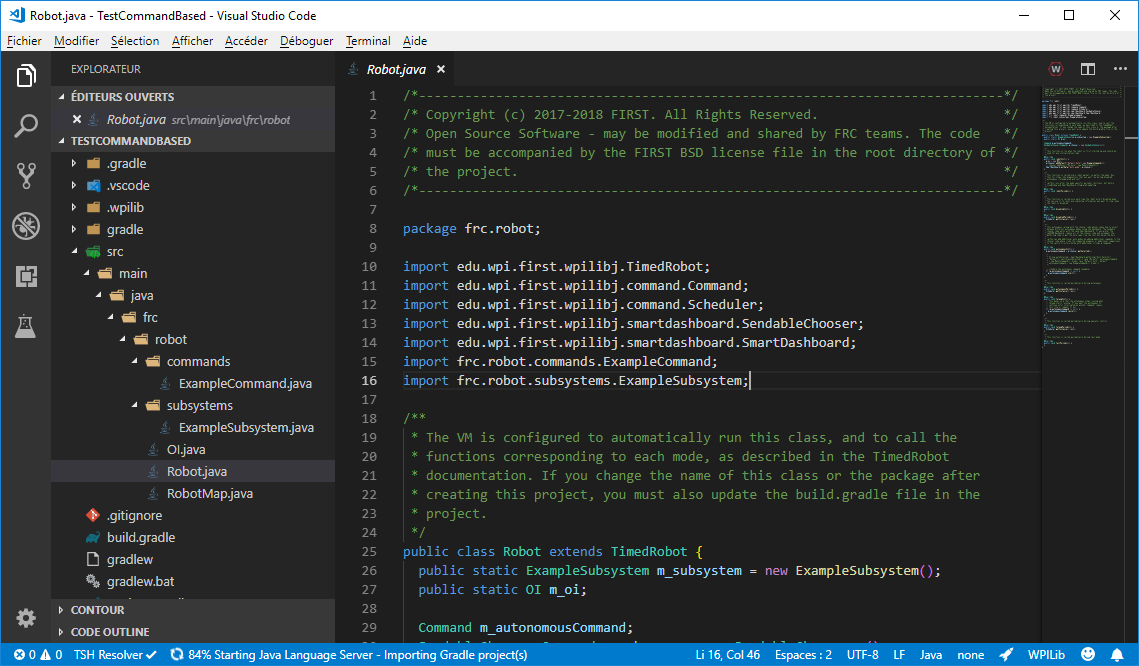
\includegraphics[width=0.9\textwidth]{creation-command-robot.png}
  \caption{La hiérarchie d'un nouveau projet \textit{Command robot}.}
\end{figure}

\section{Créer un sous-système}

\begin{enumerate}
	\item Dans le dossier \commande{src}, cliquez à droite sur le dossier \commande{subsystems}, puis sélectionnez\\ \commande{Create a new class/command}.
	\item Dans le menu affiché, sélectionnez \commande{Subsystem}.
	\item Saisissez le nom de votre sous-système. Il doit commencer par une majuscule et être sans espace.
\end{enumerate}

Comme on le faisait dans la classe \texttt{Robot}, on doit ajouter les composantes de notre sous-système dans le haut de la classe. Voici un exemple avec un sous-système nommé \texttt{Intake}, dont le rôle est de prendre et lancer un ballon.

\begin{MyTCB}[breakable]{Les attributs et le constructeur d'un sous-système}
/**
 * Sous-système de l'intake.
 * Son rôle est de prendre et relâcher un ballon.
 * Il comprend un moteur, un encodeur (pour calculer la vitesse de
 * rotation du moteur) et une limit switch, pour savoir
 * lorsqu'un ballon a été attrapé.
 */
public class Intake extends Subsystem {
  
  private VictorSP moteur;
  private Encoder encoder;
  private DigitalInput limitSwitch;

  public Intake() {

    moteur = new VictorSP(3);
    addChild("Moteur", moteur);

    encoder = new Encoder(0, 1);
    addChild("Encoder", encoder);

    limitSwitch = new DigitalInput(2);
    addChild("Limit switch", limitSwitch);

  }

  @Override
  public void initDefaultCommand() {
    // Set the default command for a subsystem here.
    // setDefaultCommand(new MySpecialCommand());
  }
  
  public void prendreBallon() {
    moteur.set(0.5);
  }
  
  public void lancerBallon() {
  	moteur.set(-0.5);
  }
  
  public void arreterMoteur() {
  	moteur.set(0.0);
  }
  
  public boolean aUnBallon() {
    return limitSwitch.get();
  }
  
  public double getVitesse() {
  	return encoder.getRate();
  }
  
}
\end{MyTCB}

\subsection{Le constructeur}

Après avoir déclaré les trois attributs dans le haut de notre classe, nous les instancions (avec \texttt{new}) dans ce qu'on appelle le \textbf{constructeur} de notre classe. Il s'agit d'une méthode publique, sans type de retour, et dont le nom est le même que la classe. Comme son nom l'indique, le constructeur est appelé lorsque notre intake sera construit dans la mémoire du RoboRIO. C'est un peu l'équivalent de \texttt{robotInit}, mais pour un sous-système. 

\begin{code}
// Le constructeur d'un sous-système
public Intake() {
	// ...
}
\end{code}

Dans le constructeur, on instancie les attributs de notre sous-système. Remarquez que pour chaque composante, on appelle également la méthode \texttt{addChild}. Son rôle est d'associer une étiquette à notre composante et de spécifier que c'est un « enfant » (\textit{child}) de notre sous-système. Cela rendra la structure de notre robot plus claire lors du débogage.

\begin{code}
// Le constructeur d'un sous-système
public Intake() {
	
	moteur = new VictorSP(3);
	addChild("Moteur", moteur);	
	// ...
}
\end{code}

\subsection{Ajouter une commande par défaut}
Lorsqu'aucune commande en cours d'exécution n'utilise un sous-système, celui-ci peut démarrer une commande automatiquement. On appelle cette commande la \textbf{commande par défaut du sous-système}. Par exemple, la commande \texttt{Piloter} est habituellement la commande par défaut du sous-système \texttt{BasePilotable}. Cependant, plusieurs sous-systèmes n'en ont pas besoin.

Pour ajouter une commande par défaut à un sous-système, il suffit d'utiliser \texttt{setDefaultCommand} dans la méthode \texttt{initDefaultCommand}.

\begin{code}
public class BasePilotable extends Subsystem {
  // ...
  @Override
  public void initDefaultCommand() {
    setDefaultCommand(new Piloter());
  }
}
\end{code}

\subsection{Ajouter des méthodes à un sous-système}
Un sous-système n'est pas complet tant qu'on ne lui ajoute pas de méthodes. Les méthodes d'un sous-système sont habituellement publiques et ont la forme suivante.

\begin{tcolorbox}[enhanced,colframe=ultRed,
	title={La déclaration d'une méthode dans un sous-système},
	sharp corners=south,
	boxsep = 1.5mm]
\texttt{{\color{ultRed}public}} {\color[RGB]{255, 34, 12} typeRetour} {\color[RGB]{12, 190, 12} nomMéthode} \texttt{() \{}\\[2pt]
	\hspace*{0.5cm} {\color[RGB]{63, 136, 197} instruction1};\\[7pt]
	\hspace*{0.5cm} ... \texttt{// Autres instructions ou calculs}\\[7pt]
	\hspace*{0.5cm} \texttt{{\color{ultRed}return}} {\color[RGB]{255, 34, 12}valeur}\texttt{;} \texttt{// Facultatif, dépend du type de retour}\\[2pt]
	\texttt{\}}
%
\end{tcolorbox}

Un sous-système a habituellement deux types de méthodes : celles qui effectuent des actions, et celles qui retournent une information. 

La majorité des méthodes qui effectuent des actions ne retournent pas d'information. Leur type de retour est donc \texttt{void}, pour indiquer qu'elles ne retournent rien.

Par exemple, on veut que notre sous-système ait comme fonctionnalité de prendre un ballon. On lui ajoute la méthode \texttt{prendreBallon()}. Pour prendre un ballon, on doit activer son moteur. Cette méthode effectue une action pure : elle n'a pas à retourner d'information. C'est pourquoi son type de retour est \texttt{void}. 

\begin{code}
public void prendreBallon() {
  moteur.set(0.5);
}
\end{code}

On veut également que notre sous-système puisse nous dire lorsqu'il a un ballon ou non. Cette méthode n'effectuera pas d'action : son rôle est uniquement de nous donner une information. Comme l'information qui nous intéresse est de type booléen, ce sera le type de retour de notre méthode. 

\begin{code}
public boolean aUnBallon() {
  return limitSwitch.get();
}
\end{code}

Pour savoir si l'intake a un ballon, il suffit de retourner l'état de notre \texttt{limit switch}.

\section{Créer une commande}

\begin{enumerate}
	\item Dans le dossier \commande{src}, cliquez à droite sur le dossier \commande{commands}, puis sélectionnez\\ \commande{Create a new class/command}.
	\item Dans le menu affiché, sélectionnez \commande{Command}.
	\item Saisissez le nom de votre commande. Il doit commencer par une majuscule et être sans espace.
\end{enumerate}

Votre classe sera créée avec plusieurs méthodes vides. Voici un exemple utilisant le sous-système que nous avons créé précédemment.

\begin{MyTCB}[breakable]{Création d'une commande}
public class PrendreBallon extends Command {
  public PrendreBallon() {
    // Use requires() here to declare subsystem dependencies
    requires(Robot.intake);
  }

  // Called just before this Command runs the first time
  @Override
  protected void initialize() {
  }

  // Called repeatedly when this Command is scheduled to run
  @Override
  protected void execute() {
    Robot.intake.prendreBallon();
  }

  // Make this return true when this Command no longer needs to run execute()
  @Override
  protected boolean isFinished() {
    return Robot.intake.aUnBallon();
  }

  // Called once after isFinished returns true
  @Override
  protected void end() {
    Robot.intake.arreterMoteur();
  }

  // Called when another command which requires one or more of the same
  // subsystems is scheduled to run
  @Override
  protected void interrupted() {
    end();
  }
}
\end{MyTCB}



\subsection{Le constructeur}
Dans le constructeur, on doit spécifier les sous-systèmes que la commande utilise. Pour ce faire, on appelle la méthode \texttt{requires} pour chaque sous-système utilisé.

\begin{code}
public LancerBallon() {
	requires(Robot.intake);
	// Autres sous-systèmes, si nécessaire
	// requires(Robot.basePilotable);
	// ...
}
\end{code}

\subsection{Cycle de vie d'une commande}
Le cycle de vie d'une commande est entièrement géré par le \texttt{Scheduler}. C'est lui qui décide quand les commandes sont démarrées et arrêtées. 
\begin{figure}[H]
\resizebox{\linewidth}{!}{%
\begin{tikzpicture}[
action/.style={rectangle, draw=green!60, fill=green!5, very thick, minimum size=7mm, text width=6cm, inner sep=0.25cm, rounded corners, align=center},
question/.style={rectangle, draw=blue!60, fill=blue!5, very thick, minimum size=7mm, text width=6cm, inner sep=0.25cm, rounded corners, align=center}
]
	\node[question] (n1)	at (0,0) {La commande est démarrée.};
	\node[action, anchor=north, shift={(0mm,-5mm)}] (n2) at (n1.south)	{\texttt{initialize()}};
	\node[action, anchor=north, shift={(0mm,-5mm)}] (n3) at (n2.south)	{\texttt{execute()}};
	\node[question, anchor=north, shift={(0mm,-5mm)}] (n4) at (n3.south)	{\texttt{isFinished()}};
	\node[question, anchor=north, shift={(0mm,-15mm)}] (n5) at (n4.south)	{Une nouvelle commande a-t-elle besoin d'un sous-système utilisé par cette commande?};
	\node[action, anchor=west, shift={(20mm,0mm)}] (n6) at (n4.east)	{\texttt{end()}};
	\node[action, anchor=west, shift={(20mm,0mm)}] (n7) at (n5.east)	{\texttt{interrupted()}};
	
	\draw[->] (n1) -- (n2);
	\draw[->] (n2) -- (n3);
	\draw[->] (n3) -- (n4);
	\draw[->] (n4) -- node[right] {\texttt{false}} (n5);
	\draw[->] (n5.west) .. controls +(left:1.5cm) and +(left:1.5cm) .. node[left] {Non} (n3.west);	
	\draw[->] (n4) -- node[above] {\texttt{true}} (n6);
	\draw[->] (n6.north) .. controls +(up:3cm) and +(right:3cm) .. ([yshift=-0.15cm]n1.east);	
	\draw[->] (n5) -- node[above] {Oui} (n7);
	\draw[->] (n7.east) .. controls +(right:2cm) and +(right:12cm) .. ([yshift=0.15cm]n1.east);	
\end{tikzpicture}}
 \caption{Le cycle de vie d'une commande.}
\end{figure}

\subsection{La méthode \texttt{initialize()}}
La méthode \texttt{initialize()} est appelé une seule fois, lorsque la commande est démarrée. C'est le bon endroit pour remettre à zéro des capteurs comme des encodeurs ou un gyro.

\begin{code}
\Override
public void initialize() {
	// On réinitialise le gyro au début de la commande
	Robot.basePilotable.resetGyro();
}
\end{code}

\subsection{La méthode \texttt{execute()}}
La méthode \texttt{execute()} est le coeur de la commande. Elle sera exécutée en boucle, tant que la commande est exécutée.

\begin{code}
\Override
public void execute() {
	// Tant que la commande s'exécute, on active le moteur pour prendre un ballon
	Robot.intake.prendreBallon();
}
\end{code}

\subsection{La méthode \texttt{isFinished()}}
Contrairement aux autres, la méthode \texttt{isFinished()} retourne un booléen. Le système s'en sert pour déterminer si une commande est terminée. Si la méthode retourne \texttt{true}, alors la commande s'arrêtera par elle-même. Sinon, elle continue, et \texttt{execute()} sera appelée une nouvelle fois. Dans notre exemple, on veut que la commande s'arrête dès que l'intake a attrapé un ballon.

\begin{code}
@Override
public boolean isFinished() {
  return Robot.intake.aUnBallon();
}
\end{code}

Dans certains cas, on veut que la commande ne se termine jamais par elle-même. C'est le cas de la commande de pilotage. Dans ce cas, on retourne toujours \texttt{false}.

\begin{code}
@Override
public boolean isFinished() {
  return false;
}
\end{code}

Si on veut que la commande se termine instantanément, il suffit de retourner \texttt{true}.

\subsection{La méthode \texttt{end()}}
La méthode \texttt{end()} est appelée lorsque la commande s'est terminée par elle-même. Par exemple, on peut donc y arrêter les moteurs qui étaient en cours d'utilisation.

\begin{code}
@Override
public void end() {
  Robot.intake.arreterMoteur();
}
\end{code}

\subsection{La méthode \texttt{interrupted()}}
La méthode \texttt{interrupted()} est appelée lorsque la commande est interrompue par une autre commande et qu'elle doit s'arrêter abruptement. Elle est souvent similaire à \texttt{end()}. On peut donc la réutiliser.

\begin{code}
@Override
public void interrupted() {
  end();
}
\end{code}

\subsection{Ajouter un délai avec \texttt{setTimeout(double) et \texttt{isTimedOut()}}}
Il est souvent utile de spécifier un délai à une commande. Par exemple, en mode autonome, on pourrait avoir besoin d'une commande qui fait avancer le robot en ligne droite pendant 3 secondes.

\begin{MyTCB}{Commande avec délai}
public class AvancerLigneDroite extends Command {
  
  public AvancerLigneDroite() {
    requires(Robot.basePilotable);
    setTimeout(3);
  }

  @Override
  protected void initialize() {
  }

  @Override
  protected void execute() {
    Robot.basePilotable.avancer();
  }

  @Override
  protected boolean isFinished() {
    return isTimedOut();
  }

  @Override
  protected void end() {
    Robot.basePilotable.arreterMoteurs();
  }

  @Override
  protected void interrupted() {
    end();
  }
}
\end{MyTCB}

On spécifie le délai dans le constructeur avec la méthode \texttt{setTimeout(double)}. Le nombre passé en paramètres correspond au délai, en secondes. La commande se terminera donc après 3 secondes.

\begin{code}
	setTimeout(3.0);
\end{code}

Il faut également vérifier si le délai a été dépassé dans la méthode \texttt{isFinished()}.

\begin{code}
@Override
protected boolean isFinished() {
  return isTimedOut();
}
\end{code}

On peut combiner un délai à une autre condition. Dans l'exemple suivant, la commande se termine si on dépasse le délai ou si on attrape un ballon.

\begin{code}
@Override
protected boolean isFinished() {
  return isTimedOut() || Robot.intake.aUnBallon();
}
\end{code}


\subsection{Lier un bouton à une commande dans la classe \texttt{OI}}
Par convention, les boutons sont liés aux commandes dans la classe \texttt{OI} (l'interface opérateur, \textit{operator interface} en anglais). 

\begin{MyTCB}{L'interface opérateur}
public class OI {

  private Joystick joystick;
  private JoystickButton button1;
  private JoystickButton button2;

  public OI() {

    joystick = new Joystick(0);

    button1 = new JoystickButton(joystick, 1);
    button1.whileHeld(new PrendreBallon());

    button2 = new JoystickButton(joystick, 2);
    button2.whenPressed(new LancerBallon());

  }

}
\end{MyTCB}

Dans un premier temps, on déclare les joysticks et les boutons comme attributs privés au haut de notre classe. Ensuite, dans le constructeur, on les instancie. Le constructeur d'un \texttt{JoystickButton} reçoit en paramètres le \texttt{Joystick} auquel il est lié et son numéro.

Pour démarrer une commande au moment où un bouton est appuyé, on utilise la méthode \texttt{whenPressed}.

\begin{code}
button2.whenPressed(new LancerBallon());
\end{code}

Dans certains cas, on veut qu'une commande soit exécutée tant qu'on maintient le bouton appuyé. On utilise alors la méthode \texttt{whileHeld}.

\begin{code}
button1.whileHeld(new PrendreBallon());
\end{code}

De plus, il est possible de démarrer une commande en appuyant sur un bouton, puis de l'annuler en réappuyant sur le même bouton. Le bouton agit alors comme un interrupteur. La méthode \texttt{toggleWhenPressed} a été créée pour répondre à ce besoin.

\begin{code}
button1.toggleWhenPressed(new PrendreBallon());
\end{code}

\section{Créer un groupe de commandes}

Les commandes simples peuvent être groupées ensemble pour former des séquences plus complexes. On les appelle des \textbf{groupes de commandes} (\textit{CommandGroup}).

\begin{enumerate}
	\item Dans le dossier \commande{src}, cliquez à droite sur le dossier \commande{commands}, puis sélectionnez\\ \commande{Create a new class/command}.
	\item Dans le menu affiché, sélectionnez \commande{Command Group}.
	\item Saisissez le nom de votre groupe de commandes. Il doit commencer par une majuscule et être sans espace.
\end{enumerate}

\begin{MyTCB}{Groupe de commandes avec addSequential}
public class LancerBallonHaut {
	
	public LancerBallonHaut() {
	
		addSequential(new LeverElevateur());
		addSequential(new LancerBallon());
		addSequential(new DescendreElevateur());
		
	}
	
}
\end{MyTCB}

Dans un groupe de commandes, il suffit d'ajouter dans le bon ordre les commandes qu'on souhaite démarrer. La méthode \texttt{addSequential} ajoute les commandes \texttt{séquentiellement}, c'est-à-dire que l'exécution du groupe est « bloquée » jusqu'à ce que la sous-commande soit terminée. Dans l'exemple ci-dessus, le robot lève l'élévateur, il lance le ballon, puis il redescend l'élévateur. Ces actions sont réalisées l'une à la suite de l'autre.

\begin{MyTCB}{Groupe de commandes avec addParallel}
public class Autonome1 {
	
	public Autonome1() {
	
		addParallel(new Avancer1metre());
		addParallel(new LeverElevateur());
		
	}
	
}
\end{MyTCB}

Contrairement à \texttt{addSequential}, la méthode \texttt{addParallel} ne bloque pas l'exécution du groupe. Les commandes s'exécutent donc \textbf{parallèlement} (en même temps). Dans cet exemple, on lève l'élévateur en même temps de faire avancer la base pilotable. Cela nous permet d'économiser du temps, ce qui est essentiel en mode autonome! Nécessairement, il faut que les commandes ajoutées en parallèle n'utilisent pas les mêmes sous-systèmes.

\begin{MyTCB}{Groupe de commandes avec WaitForChildren et WaitCommand}
public class Autonome2 {
	
	public Autonome2() {
	
		addParallel(new Avancer1metre());
		addParallel(new LeverElevateur());
		
		addSequential(new WaitForChildren());
		addSequential(new WaitCommand(2));
		
		addSequential(new LancerBallon());
		
		addParallel(new DescendreElevateur());
		addParallel(new Reculer1metre());
		
	}
	
}
\end{MyTCB}

WPILib nous fournit deux commandes très utiles : \texttt{WaitForChildren} et \texttt{WaitCommand}. \texttt{WaitForChildren} bloque l'exécution jusqu'à ce que toutes les commandes démarrées jusqu'à présent soient terminées. Dans l'exemple, on attend donc que la base pilotable ait terminé d'avancer et que l'élévateur se soit levé. Ensuite, \texttt{WaitCommand} fait attendre le robot pendant 2 secondes avant de lancer le ballon. La commande se termine en faisant reculer le robot en même temps que de faire descendre l'élévateur.

\section{Le processus de création d'une commande}

Contrairement à ce qui a été présenté jusqu'à présent, il est rare que l'on sait exactement les méthodes dont un sous-système aura besoin avant de créer une commande. 

\begin{figure}[H]
\resizebox{\linewidth}{!}{%
\begin{tikzpicture}[
action/.style={rectangle, draw=green!60, fill=green!5, very thick, minimum size=7mm, text width=6cm, inner sep=0.25cm, rounded corners},
question/.style={rectangle, draw=blue!60, fill=blue!5, very thick, minimum size=7mm, text width=6cm, inner sep=0.25cm, rounded corners}
]
	\node[action] (n1)	at (0,0)	{Créer un fichier pour la commande.};
	%\node[action, anchor=north, shift={(0mm,-5mm)}] (n2) at (n1.south)	{Appeler \texttt{super("...")} dans le constructeur pour donner un nom à la commande.};
	\node[question, anchor=north, shift={(0mm,-5mm)}] (n3)  at (n1.south)	{Déterminer les sous-systèmes que la commande va utiliser. Est-ce que je dois en ajouter un nouveau?};
	\node[action, anchor=west, shift={(20mm,0mm)}] (n4) at (n3.east)	{Créer un fichier pour le sous-système.};
	% \node[action, anchor=north, shift={(0mm,-5mm)}] (n5) at (n4.south)	{Appeler \texttt{super("...")} dans le constructeur pour donner un nom au sous-système.};
	\node[action, anchor=north, shift={(0mm,-5mm)}] (n6) at (n4.south)	{Ajouter les composantes du sous-système comme attributs privés (\texttt{private}).};
	\node[action, anchor=north, shift={(0mm,-5mm)}] (n7) at (n6.south)	{Instancier (\texttt{new} et \texttt{addChild}) les composantes dans le constructeur et ajouter les ports nécessaires à la classe \texttt{K}.};
	\node[action, anchor=north, shift={(0mm,-5mm)}] (n8) at (n7.south)	{Ajouter le sous-système dans le haut de classe Robot comme attribut public statique final.};
	\node[action, anchor=north, shift={(0mm,-10mm)}] (n9)  at (n3.south)	{Appeler la méthode \texttt{require(subsystem)} pour chaque sous-système dans le constructeur de la commande.};
	\node[question, anchor=north, shift={(0mm,-5mm)}] (n10)  at (n9.south)	{Déterminer les sous-actions que la commande va faire et les informations dont elle aura besoin. Vérifier si les sous-systèmes ont des méthodes qui correspondent à ces besoins. Est-ce que je dois créer une nouvelle méthode?};
	\node[action, anchor=north, shift={(0mm,-10mm)}] (n11) at (n10.south) {Compléter la commande en utilisant les méthodes des sous-systèmes requis. Utiliser \texttt{setTimeout(double)} et \texttt{isTimedOut()} si nécessaire.};
	\node[action, anchor=north, shift={(0mm,-5mm)}] (n12) at (n11.south) {Ajouter votre commande dans l'\texttt{OI} (par exemple, à un bouton ou sur le SmartDashboard).};
	\node[action, anchor=north, shift={(0mm,-5mm)}] (n13) at (n12.south) {Tester!};
	\node[action, anchor=east, shift={(-20mm,0mm)}] (n14) at (n10.west)	{Aller dans le fichier du sous-système correspondant.};
	\node[action, anchor=north, shift={(0mm,-5mm)}] (n15) at (n14.south)	{Créer une méthode publique dans la classe. Si la commande a besoin d'une information, le type de retour doit être le même que l'information (par exemple, \texttt{double} si hauteur, \texttt{boolean} si état d'une \textit{switch}). Si la méthode effectue une action pure, la méthode ne retourne rien et est de type \texttt{void}. N'oubliez d'effectuer des vérifications, si nécessaire, et d'ajouter des constantes dans la classe \texttt{K}.};
	% \draw[->] (n1) -- (n2);
	\draw[->] (n1) -- (n3);
	\draw[->] (n3) -- node[above] {Oui} (n4);
	% \draw[->] (n4) -- (n5);
	\draw[->] (n4) -- (n6);
	\draw[->] (n6) -- (n7);
	\draw[->] (n7) -- (n8);
	\draw[->] (n8.west) .. controls +(left:2cm) and +(right:2cm) .. ([yshift=-0.35cm]n3.east);
	\draw[->] (n3) -- node[right] {Non} (n9);
	\draw[->] (n9) -- (n10);
	\draw[->] (n10) -- node[right] {Non} (n11);
	\draw[->] (n11) -- (n12);
	\draw[->] (n12) -- (n13);
	\draw[->] (n10) -- node[above] {Oui} (n14);
	\draw[->] (n14) -- (n15);
	\draw[->] (n15.east) .. controls +(right:2cm) and +(left:2cm) .. ([yshift=-0.8cm]n10.west);
\end{tikzpicture}}
\caption{Le processus de création d'une commande.}
\end{figure}

\begin{figure}[H]
\resizebox{\linewidth}{!}{%
\begin{tikzpicture}[
action/.style={rectangle, draw=green!60, fill=green!5, very thick, inner sep=0.25cm, rounded corners, align=left},
question/.style={rectangle, draw=blue!60, fill=blue!5, very thick, inner sep=0.25cm, rounded corners}
]
\draw [decorate,decoration={brace,mirror,amplitude=5pt}] (0, -0.1) -- (0, -1.9) node[midway,left,xshift=-0.5cm] {OI et Autonome};
\draw [decorate,decoration={brace,mirror,amplitude=5pt}] (0,-2.1) -- (0,-3.9) node[midway,left,xshift=-0.5cm] {Commandes};
\draw [decorate,decoration={brace,mirror,amplitude=5pt}] (0,-4.1) -- (0,-5.9) node[midway,left,xshift=-0.5cm] {Méthodes};
\draw [decorate,decoration={brace,mirror,amplitude=5pt}] (0,-6.1) -- (0,-7.9) node[midway,left,xshift=-0.5cm] {Attributs};
\draw [decorate,decoration={brace,mirror,amplitude=8pt}, xshift=-0.5cm,yshift=0pt] (-3,-4.1) -- (-3,-7.9) node[midway,left,xshift=-0.5cm] {Sous-systèmes};

\node[action] (n1) at (3,-1) {Bouton A};
\node[action] (n2) at (9,-1) {Autonome};

\node[action] (n3) at (3,-3) {\texttt{TirerBallon}};
\node[action] (n4) at (9,-3) {\texttt{Autonome(distance)}};

\node[action] (n5) at (3,-5) {\texttt{shoot()}};
\node[action] (n6) at (17,-5) {\texttt{arcadeDrive(forward, rotation)}};
\node[action] (n7) at (9,-5) {\texttt{getDistance()}};

\node[action] (n8) at (3,-7) {\texttt{moteur.set(0.6)}};
\node[action, text width=5.8cm] (n9) at (9,-7) {\texttt{encoderGauche.getDistance() encoderDroit.getDistance()}};
\node[action, text width=5.8cm] (n10) at (17,-7) {\texttt{drive.arcadreDrive(f, r)}};

\draw[->] (n1) -- (n3);
\draw[->] (n2) -- (n4);
\draw[->] (n3) -- (n5);
\draw[->] (n4) -- (n6);
\draw[->] (n4) -- (n7);
\draw[->] (n5) -- (n8);
\draw[->] (n7) -- (n9);
\draw[->] (n6) -- (n10);

\end{tikzpicture}}
\caption{La séquence d'appels dans un programme WPILib.}
\end{figure}


\end{document}
